\documentclass{article}
\usepackage{graphicx} % Required for inserting images
\usepackage[round]{natbib}
\usepackage{amsmath, amssymb}
\usepackage{dsfont}
\usepackage[noend]{algpseudocode}
\usepackage{algorithm}
\usepackage{bbm}
\usepackage{pdfpages}
\usepackage{float}
\usepackage[a4paper]{geometry}
\usepackage[T1]{fontenc}
\usepackage{ifthen}


\usepackage{listings}
\usepackage{tcolorbox}
\usepackage{tikz}
\usepackage{pgfplots}
\usepackage{pgfplotstable}
\usepackage{xcolor}
\usepackage{caption}
\usetikzlibrary{pgfplots.colorbrewer}

\newcommand{\lstfont}[1]{\color{#1}\scriptsize\ttfamily}

\lstset{
    language=[ANSI]C++,
    showstringspaces=false,
    backgroundcolor=\color{white!90},
    basicstyle=\lstfont{black},
    identifierstyle=\lstfont{black},
    keywordstyle=\lstfont{purple},
    commentstyle=\lstfont{green!50!black},
    emph={
        cudaMalloc, cudaFree,
        __global__, __shared__, __device__, __host__,
        __syncthreads, cudaDeviceSynchronize, pragma, unroll
    },
    emphstyle={\lstfont{blue}},
    breaklines=true
}

\usepackage{tikz}
\usetikzlibrary{decorations.pathreplacing}
\usetikzlibrary{plotmarks}

\usepackage{pgfplots}
\usepackage{pgfplotstable}
\usepgfplotslibrary{external}
\pgfplotsset{compat=1.5}

\usepackage{xcolor}
\newcommand\todo[1]{\textcolor{red}{#1}}

\newcommand\R{\mathds{R}}

\newcommand{\resultplot}[5]{%
    \pgfplotsset{
        % initialize Set1-5:
        cycle list/Set3-12,
        % combine it with 'mark list*':
        cycle multiindex* list={
            mark list*\nextlist
            Set3-12\nextlist
        },
    }
    \pgfplotstableread[col sep=comma]{#2}\accutable
    \pgfplotstableread[col sep=comma]{#3}\timetable

    \begin{minipage}{\textwidth}
        \begin{tikzpicture}
            \begin{axis}[
                    name=timeax,
                    xmajorgrids=true, ymajorgrids=true,
                    xlabel={Noise}, ylabel={Accuracy},
                    xtick=data,
                    xticklabels={0, 5, 10, 15, 20, 25},
                    %legend style={at={(0.5,-0.16)}, anchor=north, legend columns=2, font=\footnotesize, legend cell align={left}},
                    width=\textwidth*0.45,
                    height=\textwidth*0.45,
                ]
                \pgfplotsforeachungrouped \i in {0,...,#4} {
                    \addplot table[x expr=\coordindex, y index=\i] 
                    {\accutable};
                }
                %\legend{\textsc{Fugal}, \textsc{CugalMix}, \textsc{CugalMix} $\gamma$0.1, \textsc{CugalMix} $\gamma$0.2,\textsc{CugalMixGreedy}, \textsc{CugalMixGreedy} $\gamma$0.1, \textsc{CugalMixGreedy} $\gamma$0.2,\textsc{CugalLog}, \textsc{CugalLog} $\gamma$0.1, \textsc{CugalLog} $\gamma$0.2, \textsc{CugalLogGreedy}, \textsc{CugalLogGreedy} $\gamma$0.1, \textsc{CugalLogGreedy} $\gamma$0.2}
            \end{axis}
            \begin{semilogyaxis}[
                    at={(timeax.south east)},
                    xshift=2cm,
                    xmajorgrids=true, ymajorgrids=true,
                    xlabel={Noise}, ylabel={Time (s)},
                    xtick=data,
                    xticklabels={0, 5, 10, 15, 20, 25},
                    legend style={at={(-0.25,-0.1)}, anchor=north, legend columns=3, font=\footnotesize, legend cell align={left}},
                    width=\textwidth*0.45,
                    height=\textwidth*0.45,
                ]
                \pgfplotsforeachungrouped \i in {0,...,#4} {
                    \addplot table[x expr=\coordindex, y index=\i] 
                    {\timetable};
                }
                \ifthenelse{\equal{#5}{true}}{
                \legend{\textsc{Fugal}, \textsc{cuGAL-Mix}, \textsc{cuGAL-Mix} $\gamma=0.1$, \textsc{cuGAL-Mix} $\gamma=0.2$,\textsc{cuGAL-Mix-Greedy}, \textsc{cuGAL-Mix-Greedy} $\gamma=0.1$, \textsc{cuGAL-Mix-Greedy} $\gamma=0.2$,\textsc{cuGAL-Log}, \textsc{cuGAL-Log} $\gamma=0.1$, \textsc{cuGAL-Log} $\gamma=0.2$, \textsc{cuGAL-Log-Greedy}, \textsc{cuGAL-Log-Greedy} $\gamma=0.1$, \textsc{cuGAL-Log-Greedy} $\gamma=0.2$}
                }{}
            \end{semilogyaxis}
        \end{tikzpicture}
        \captionof{figure}{Runtime and accuracy on #1 dataset}
        \label{fig:#1_res}
    \end{minipage}
}



\usepackage{hyperref}
\hypersetup{
    colorlinks=true,
    linkcolor=blue,
    filecolor=magenta,      
    urlcolor=cyan,
    citecolor=black,
}


\title{cuGAL: Graph Alignment on the GPU}
\author{Sebastian Rue Clausen, Andreas H. H. Hansen}
\date{\today}

\begin{document}

\begin{titlepage}
    \maketitle
    \centering
    \begin{tikzpicture}[scale=2]
    % Graph 1 nodes
    \path
    (1, 0) node[circle, draw] (A1) {}
    (0, 1) node[circle, draw] (B1) {}
    (2, 1) node[circle, draw] (C1) {}
    (1, 2) node[circle, draw] (D1) {}
    (0, 3) node[circle, draw] (E1) {}
    (2, 3) node[circle, draw] (F1) {}
    (1, 4) node[circle, draw] (G1) {}
    ;

    % Graph 1 edges
    \draw (A1) -- (B1);
    \draw (A1) -- (C1);
    \draw (B1) -- (C1);
    \draw (B1) -- (D1);
    \draw (C1) -- (D1);
    \draw (C1) -- (F1);
    \draw (D1) -- (E1);
    \draw (D1) -- (F1);
    \draw (E1) -- (G1);

    % Graph 2 nodes (rotated)
    \path
    (5, 1) node[circle, draw] (A2) {}
    (6, 2) node[circle, draw] (B2) {}
    (4, 2) node[circle, draw] (C2) {}
    (5, 5) node[circle, draw] (D2) {}
    (5, 4) node[circle, draw] (E2) {}
    (6, 3) node[circle, draw] (F2) {}
    (4, 4) node[circle, draw] (G2) {}
    ;

    % Graph 2 edges
    \draw (A2) -- (B2);
    \draw (A2) -- (C2);
    \draw (B2) -- (C2);
    \draw (B2) -- (D2);
    \draw (C2) -- (D2);
    \draw (C2) -- (F2);
    \draw (D2) -- (E2);
    \draw (D2) -- (F2);
    \draw (E2) -- (G2);

    % Matching edges
    \draw[dashed] (A1) -- (A2);
    \draw[dashed] (B1) -- (B2);
    \draw[dashed] (C1) -- (C2);
    \draw[dashed] (D1) -- (D2);
    \draw[dashed] (E1) -- (E2);
    \draw[dashed] (F1) -- (F2);
    \draw[dashed] (G1) -- (G2);

\end{tikzpicture}
\end{titlepage}

\section*{Abstract}
Graph alignment is an NP-hard problem, making good approximations computationally expensive for large graphs. Recent developments indicate that working directly with adjacency matrices yields better results compared to other methods. In this report, we propose \textsc{cuGAL}, an accelerated version of the state-of-the-art algorithm \textsc{Fugal}, utilizing GPU technology. Our modifications enhance the scalability of \textsc{Fugal} while maintaining its high accuracy. We implement \textsc{cuGAL} efficiently using CUDA and extensively benchmark it against \textsc{Fugal}. Our results demonstrate significant improvements in both accuracy and speed for large graph datasets.

\tableofcontents

\section{Introduction}
Graphs are powerful and widely used data structures for modelling relationships between entities. They are employed to represent a wide range of systems, from road networks and social relations to biological systems and protein structures. Many algorithms have been developed to analyse and solve graph-related problems, among which is the problem of graph alignment. Graph alignment involves mapping nodes between two graphs to maximise a measure of similarity. This is often used to find matching entities in two graphs, such as the same persons in two social networks \citep{koutra2013big}, the same protein in two biological structures \citep{singh2008isorank} or image features in computer vision \citep{conte2003graph}. Due to the NP-hardness of the problem, algorithms will have to approximate an answer. To be applicable in a wide range of use cases, algorithms will also have to be resistant to noise, meaning no perfect mapping exists between the graphs.\\

In this project, we aim to improve the speed of an existing algorithm \textsc{Fugal} \citep{fugal2024} while maintaining its excellent accuracy compared to other algorithms. Although \textsc{Fugal} scales well compared to similar algorithms, performance remains a problem for larger graphs. We propose using GPUs (Graphical Processing Units) to take advantage of the parallelisable nature of the \textsc{Fugal} algorithm. We create an efficient GPU implementation of \textsc{Fugal} that takes advantage of modern GPU hardware. In addition, we make several modifications based on extensive analysis of \textsc{Fugal}, to further improve scalability for large graphs. We call our algorithm \textsc{cuGAL} - a combination of CUDA and \textsc{FUGAL}.\\

Throughout the project, we focus on different steps of the algorithm. We analyse each step and propose optimisations based on our findings. We then benchmark our implementation to test both accuracy and speed compared to \textsc{Fugal}.

\section{Background}
\subsection{The Graph Alignment Problem}
%Something general
The graph alignment problem involves finding a bijective function $f: V_1 \rightarrow V_2$, that maps each node in graph $G_1 = (V_1, E_1)$ to each node in graph $G_2 = (V_2, E_2)$. The objective is to find a mapping such that a similarity of the connected nodes is maximised. The measure of similarity may vary dependent on the problem being solved.\\

\noindent
\textbf{Unrestricted:} The objective of \textsc{Fugal} is the problem of \textit{unrestricted} graph alignment. \textit{Unrestricted} graph alignment only considers the topology of the graph to determine an alignment. Given adjacency matrices $A$ and $B$ of $G_1$ and $G_2$ respectively, we find a permutation such that the number of edge disagreements is minimised:

\begin{equation}\label{original_qap}
\min_{P \in \mathds{P}^n} \lVert AP-PB \rVert^2_F
\end{equation}

where $\mathds{P}^n$ is a $n \times n$ permutation matrices. This is an instance of QAP (Quadratic assignment problem) \citep{fan2020spectral}, which is NP-hard \citep{sahni1972qap}.\\

\noindent
\textbf{Restricted:} For \textit{restricted} graph alignment, an alignment is determined based on both graph topology and vertex features. This may be required to sufficiently model real world problems. We further expand on this in Chapter \ref{related_work}.

\subsection{Approaches to Graph Alignment}
Existing algorithm tackle the graph alignment problem in very different ways. \cite{fugal2024} splits these into two categories:\\

\noindent
\textbf{Mediated:} Algorithms that take a \textit{mediated} approach to graph alignment, compute graph representations of $G_1$ and $G_2$, which is used to compute similarity scores between nodes. By stating this as a LAP (Linear Assignment Problem), an alignment can be found in polynomial time. We go further into detail on \textit{mediated} graph alignment in Chapter \ref{related_work}.\\

\noindent
\textbf{Unmediated:} For \textit{unmediated} graph alignment, algorithms work directly with the adjacency matrices of $G_1$ and $G_2$. This has the advantage that algorithms can base their alignment on the full and unmediated structure of the graphs. \textit{Unmediated} approaches can more directly tackle the QAP of \textit{unrestricted} graph alignment (Equation \ref{original_qap}). The algorithms of \citep{vogelstein2015fast} and \citep{fugal2024} both relaxes the constraints of the QAP to find an approximation in polynomial time. Both generally achieves excellent results compared to \textit{mediated} approaches. \citep{fugal2024} shows that an \textit{unmediated} approach also can be feasible for relatively large graphs.


\iffalse
\noindent
\textbf{Input:} The algorithm may work with either \textit{unrestricted} or \textit{restricted} graph alignment. With \textit{unrestricted} graph alignment, only the topology of the graphs are considered. An example of a problem where this would be useful, is for modelling relationships. For other problems, such as modelling biological networks \citep{singh2008isorank}, \textit{restricted} graph alignment is often used, see \ref{related_work}\\

\noindent
\textbf{Representation:} An algorithm must decide on a representation of the graphs. % popular representation is node embeddings. This nodes in relation to the topology of the graph. Embeddings may also contain information about the node features. This is at times referred to as \textit{mediated} graph alignment. The problem can now be solved by mapping similar embeddings, which can be solved in polynomial time. Algorithms such as GRAAL \citep{kuchaiev2010topological}, REGAL \citep{bayati2009algorithms} and CONE \citep{chen2020cone} all use embeddings in various ways. 
One option is to work with adjacency matrices directly, called \textit{unmediated} graph alignment. This can be computationally expensive, as adjacency matrices become large, but allows the algorithm to have access to the full topology of the graphs. Algorithms such as \textsc{Fugal} \citep{fugal2024} and \textsc{Faq} \citep{vogelstein2015fast} work in this manner.\\

%Lastly, the method used for assignment must be chosen. This is the method which, based on the similarity found before, chooses which pairs of nodes should be matched between the two bipartite graphs. This can be done through a variety of means, depending on the previous steps an algorithm has taken. Examples include assigning one node at a time, either greedily choosing nodes of highest similarity, using a sorting or a nearest neighbor approach, which repeatedly assigns the unmatched node with the highest similarity, or algorithms which directly solve the LAP, like the Hungarian algorithm or Maximum Weighted Matching (\cite{skitsas2023GAEval, fugal2024})
\fi

\subsection{GPU computation}
Although GPUs (Graphical Processing Units) were originally developed for processing 3D graphics, today they are often used to speed up computationally expensive and parallelizable tasks. The use of GPUs for general computation has become increasingly prevalent since the early 2000s. This has especially been the case for linear algebra operations such as matrix multiplication \citep{gpgpu2007}, which now powers the explosive success of deep learning. With the development of the CUDA programming framework from NVIDIA, programmers have been able exploit the raw compute power of increasingly powerful GPUs with relative ease.

GPUs are able to achieve their impressive compute throughput by being able to run vastly more threads concurrently compared to CPUs. However, utilising the threads optimally remains a significant challenge even for easily parallizable problems. Therefore, porting algorithms to GPUs requires many considerations about managing threads and memory, including transferring memory between GPU and CPU memory and keeping threads busy.

\subsection{Graphs}
We test on a large variety of both synthetic and real world graphs. When testing, we always permute the indices of the nodes of $G_2$ using a random permutation $\sigma : V_2 \rightarrow V_2$:
\begin{equation}
    G_2 \gets (V_2, \{ (\sigma(i), \sigma(j)) \vert (i, j) \in E_2 \})    
\end{equation}

When testing with no noise, then $E_1 = E_2$. We work with two main categories of noise: real noise and synthetic noise. With real noise, $G_1$ and $G_2$ are two different but related graphs. For synthetic noise, we use one of the noise types defined by \cite{skitsas2023GAEval}, namely \textit{one-way} noise, defined as randomly removing a percentage $t \in [0, 1]$ of edges from $G_2$:
\begin{equation}
    E_2 \gets E_2 \setminus \textit{Sample}(E_2, t)
\end{equation}

We choose to only evaluate a single metric of quality, namely accuracy. We define the accuracy of a mapping $f : V_1 \rightarrow V_2$ as:
\begin{equation}
    \frac{1}{|V_1 \cap V_2|} \sum_{i \in V_1 \cap V_2} \begin{cases}
        1 & \sigma(i) = f(i)\\
        0 & \sigma(i) \neq f(i)\\
    \end{cases} 
\end{equation}

Throughout the report, we test on graphs from the following datasets:

\begin{table}[htbp]
\begin{center}
\begin{tabular}{ |l|r|r| } 
 \hline
 \textbf{Graph} & $n$ & $m$ \\ 
 \hline
 Newmann-Watts (NW) \citep{newman2001random} & - & - \\ 
 ASTRO-PH \citep{leskovec2007graph} & 17 903 & 197 031 \\ 
 HEP-PH \citep{kosowska2016evolving} & 12 008 & 118 521 \\ 
 inf-euroroad \citep{bader2012graph} & 1 174 & 1 417 \\ 
 email-Enron \citep{leskovec2009community} & 36 692 & 183 831 \\ 
 bio-dmela \citep{nr2015} & 7 393 & 25 569 \\
 vole \citep{davis2014spatial} & 712 & 2 391 \\
 MultiMagna \citep{vijayan2017multiple} & 1 004 & 8 323 \\
 inf-power \citep{nr2015} & 4 941 & 6 594\\
 ca-GrQc \citep{nr2015} & 4 158 & 14 422\\
 ca-netscience \citep{nr2015} & 379 & 5 818\\
 Arenas \citep{kunegis2013konect} & 1 133 & 5 451\\
 \hline
\end{tabular}
\end{center}
\caption{$n$ is the number of nodes, $m$ is the number of edges. Note that Newmann-Watts is a synthetic graph which we generate with specified parameters dependent on the use case. All graphs are undirected.}
\end{table}


\section{Related Work}\label{related_work}
Graph alignment is used to solve a large variety of real world problems. \cite{singh2008isorank} aligns proteins across multiple biological networks, using both graph structure and node similarity scores, making it an example of using \textit{restricted} graph alignment to solve real problems. \cite{kazemi2015growing} presents an algorithm to identify users across social networks based on a set of pre-aligned nodes, which can be perceived as node features. \cite{zhang2016final} presents a general purpose graph alignment algorithm \textsc{Final}, that takes advantage of edge and node attributes, and shows that edge and node information can compliment graph topology in finding an alignment. While edge and node attributes can be useful for solving real problems, \textit{unrestricted} algorithms are often able to be modified to take advantage of edge and node attributes and allows researchers to better compare different algorithms.\\

The \textit{mediated} graph alignment approach has been the predominant paradigm in recent literature. Notable algorithms employing this approach include \textsc{CONE} \citep{chen2020cone}, which utilizes Graph Neural Networks to compute node embeddings, and \textsc{REGAL} \citep{heimann2018regal}, which learns embeddings based on graph structure. \textsc{GRAAL} \cite{kuchaiev2010topological} leverages frequent patterns in graphs, while \textsc{GRASP} \citep{hermanns2021grasp} and \textsc{LREA} \citep{nassar2018low} use spectral analysis. A comprehensive evaluation by \cite{skitsas2023GAEval} examines a wide range of state-of-the-art graph alignment algorithms, all classified as mediated according to the definition by \cite{fugal2024}. The study shows significant variance in the accuracy and ranking of these algorithms, depending on the specific graph and noise level.\\

Accelerating graph algorithms using GPUs is a widely studied technique. A survey by \cite{shi2018graph} gives an overview of a wide array of algorithms and techniques used to adapt algorithms to GPU hardware. Also the problem of graph alignment has been explored on GPUs. We are aware of two examples, \textsc{cuAlign} \citep{xiang2023cualign} and \textsc{SLOTAlign} \citep{tang2023robust}, both of which uses GPUs to scale graph alignment to larger graphs.


\section{\textsc{FUGAL}}

We now describe the \textsc{Fugal} \citep{fugal2024} algorithm in detail.

\subsection{Background}
In this section, we introduce the mathematical foundations of the \textsc{Fugal} algorithms.
\subsubsection{Permutation and Doubly Stochastic matrices}
Doubly stochastic matrices are square matrices where each row and column sums to 1. More formally for matrix $X \in \mathds{R}^{n \times n}$, $\sum_{i = 1} X_{i,j} = 1$ for $j = 1, 2, .., n$ and $\sum_{j = 1} X_{i,j} = 1$ for $i = 1, 2, .., n$. Doubly stochastic matrices can be shown to be convex using the Birkhoff-von Neumann Theorem \citep{birkhoff1946three}.

Permutation matrices are a subset of doubly stochastic matrices, where each row and column only has a single non-zero entry. This means that for $X \in \mathds{P}^n$ where $\mathds{P}^n$ is the set of permutation matrices, then:

\begin{equation}\label{perm_def}
    \text{trace}(X^T(1^{n \times n}-X)) = 0
\end{equation}

Unlike doubly stochastic matrices, permutation matrices are not convex.%, which is easy to demonstrate: Consider two permutation matrices, one of them the identity matrix and another which swap two arbitrary rows. Taking the average of the two, we see that we get a doubly stochastic matrix, which is not a permutation matrix. This violates convexity. \citep{} 

\subsubsection{Quadratic Assignment Problem}
\cite{koopmans1957assignment} define the QAP (Quadratic Assignment Problem). QAP is the problem of assigning $n$ facilities to $n$ locations, given weight $W \in \mathds{R}^{n \times n}$ between facilities and distance $D \in \mathds{R}^{n \times n}$ between locations. More formally:
$$ \min_{f \in N \rightarrow N} \sum_{a=1}^n \sum_{b=1}^n W_{a, b} D_{f(a), f(b)} $$
where  $N = \{ 1, 2, .., n \}$ and $f$ is a bijective function that maps facilities to locations. This is shown to be NP-hard \citep{sahni1972qap}. By representing the mapping as permutation matrix $P$, we can express the problem as:
$$ \min_{P \in \mathds{P}^n} \lVert WP - PD \rVert_{F}^2 $$
\cite{edwards1980branch} proposes the following formulation:
\begin{equation}\label{qap_trace_rewrite}
\min_{P \in \mathds{P}^n} \lVert WP - PD \rVert_{F}^2 = \min_{P \in \mathds{P}^n} \text{trace}(WPDP^T)
\end{equation}
%https://www.sciencedirect.com/topics/computer-science/quadratic-assignment-problem
%https://link.springer.com/chapter/10.1007/BFb0120905

\subsubsection{Linear Assignment Problem}
LAP (Linear Assignment Problem) is the problem of assigning $n$ agents to $n$ tasks, where assigning agent $a$ to task $b$ has cost $W_{a,b}$. More formally:
\begin{equation}\label{lap_sum}
    \min_{P \in \mathds{P}^n} \sum_{a=1}^n \sum_{b=1}^n W_{a, b} P_{a,b}
\end{equation}
where $P$ is a permutation matrix of the mapping from agent to task. LAP can be solved in $O(n^3)$ by the Hungarian algorithm \citep{kuhn1955hungarian}. By defining the cost as the Euclidean distance between the rows of $A, B \in \mathds{R}^{n \times k}$:
\begin{equation}\label{euclidean_distance_matrix}
D_{i,j} = \sqrt{\sum^k_{m = 1} (A_{i, m} - B_{j, m})^2}
\end{equation}

we can express the problem as:
\begin{equation}\label{lap_trace_rep}
     \min_{P \in \mathds{P}^n} \lVert A - PB \rVert_{F}^2 = \min_{P \in \mathds{P}^n} \text{trace}(P^TD)
\end{equation}

\subsubsection{Optimal Transport}
OTP (Optimal Transport Problem), in the discrete case, is the problem of transforming discrete probability distributions or histograms $r \in \mathds{R}^n$ into $c \in \mathds{R}^n$ where $C \in \mathds{R}^{n \times n}$ is the cost, such that moving value from $r_i$ to $c_j$ has cost $C_{i, j}$. This may be expressed as:
\begin{equation}
    \min_{P \in U(r, c)} \langle P, C \rangle \\  
\end{equation}
where
\begin{equation}
    U(r, c) = \{ P \in \mathds{R}^{n \times n} | P\boldsymbol{1} = r, P^T\boldsymbol{1} = c \}
\end{equation}

$P$ is referred to as the transport plan as $P_{i, j}$ indicates the amount of value transferred from $r_i$ to $c_j$. This is a linear problem, and can thus be solved by the simplex method. However, this is slow in practice when $n$ is large. \cite{cuturi2013sinkhorn} proposed the introduction of the regularisation term $-\epsilon H(P)$, where $H(P)$ is the entropy between entries in $P$:
\begin{equation}
    H(P) = -\sum^{n}_{i = 1} \sum^{n}_{j = 1} P_{i, j} \log P_{i, j}
\end{equation}
The problem now becomes:
\begin{equation}
    \min_{P \in U(r, c)} \langle P, C \rangle - \epsilon H(P)
\end{equation} 
which \cite{cuturi2013sinkhorn} shows to be equivalent to the optimal transport problem for small values of $\epsilon$. \cite{cuturi2013sinkhorn} goes on to show that this can be solved efficiently using the Sinkhorn-Knopp algorithm \citep{sinkhorn1967concerning}.

\iffalse
\begin{figure}[h]
    
\includegraphics[scale=3]{figures/optimal_transport.pdf}
    \centering
    \caption{$r$ (left) being transformed into $c$ (right). The lines are a visual representation of the transport plan ($P$).}
\end{figure}
\fi

\subsubsection{Sinkhorn-Knopp}
The Sinkhorn-Knopp algorithm \citep{sinkhorn1967concerning} finds $n \times n$ diagonal matrices $D_1, D_2$ given $A \in \mathds{R}^{n \times n}$ such that the rows and columns of $D_1 A D_2$ sums to $a$ and $b$ respectively. The algorithm iteratively switches between scaling the rows and columns of $A$ until convergence.

\begin{algorithm}[H]
\caption{Sinkhorn-Knopp}\label{alg:Sinkhorn-Knopp}
\textbf{Input} $A \in \mathds{R}^{n \times n}, a, b \in \mathds{R}^{n}, \epsilon \in \mathds{R}$
\begin{algorithmic}[1]
\State $u \gets \frac{1}{n} \cdot \boldsymbol{1}$
\State $v \gets \frac{1}{n} \cdot \boldsymbol{1}$
\State $K \gets \exp(-A / \epsilon)$

\For{$i \gets 1, .., it$}
    \State $v \gets \frac{b}{uK}$
    \State $u \gets \frac{a}{Kv}$
    \If {stop condition met}
        \State \textbf{break}
    \EndIf
\EndFor

\State \Return $\text{diag}(u) K \text{diag}(v)$

\end{algorithmic}
\end{algorithm}

Different stopping conditions can be used. A common option is checking whether the row and column sums of $\text{diag}(u) K \text{diag}(v)$ is close to $a$ and $b$. Typically, some upper bound $it$ is also determined.

\subsubsection{Frank-Wolfe}
The Frank-Wolfe algorithm \citep{frank1956algorithm} is an iterative algorithm for minimising a differentiable function $f(x)$ within a convex set $D$. The algorithm transforms the problem into a linear optimisation sub-problem, which it uses to find an extreme point in $D$ roughly in the direction of $-\nabla f(x)$:
\begin{equation}
    \min_{v^{(k)} \in D} \langle \nabla f(x^{(k)}), v^{(k)} \rangle
\end{equation}

It determines $x^{(k + 1)}$ to be a linear interpolation between $v^{(k)}$ and $x^{(k)}$ using coefficient $\alpha^{(k)} \in [0, 1]$:
\begin{equation}
    x^{(k + 1)} = (1 - \alpha^{(k)})x^{(k)} + \alpha^{(k)} v^{(k)}
\end{equation}

The convexity of $D$ ensures that $x^{(k + 1)} \in D$. Various strategies can be used to determine $\alpha$. A common choice is $\alpha^{(k)} = \frac{2}{k + 2}$.
\begin{figure}[h]
    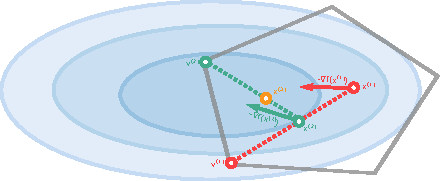
\includegraphics[scale=1.5]{figures/frank_wolfe_cropped.pdf}
    \centering
    \caption{Visual representation of two iterations of Frank-Wolfe. Here the ovals represent the gradient and the pentagon the convex bounds of the problem.}
\end{figure}

\subsection{The \textsc{Fugal} algorithm}
\textsc{Fugal} approximates an optimal alignment of graphs $G_1$ and $G_2$, by constructing an optimisation problem based on \textit{unmediated} representations of the graphs. Based upon the theoretical background described above, we now derive the \textsc{Fugal} algorithm.\\

\noindent
\textbf{QAP Term:} We start with the quadratic assignment problem from Equation \ref{original_qap}:
\begin{equation}
    \min_{P \in \mathds{P}^n} \lVert AP-PB \rVert^2_F
\end{equation} 
where $A$ and $B$ are the adjacency matrices of $G_1$ and $G_2$ respectively. Solving for $P \in \mathds{P}^n$ is NP-hard, as $\mathds{P}^n$ is non-convex \citep{koopmans1957assignment}. By expanding from $P \in \mathds{P}^n$ to the superset $P \in \mathds{W}^n$, where $\mathds{W}^n$ is the set of \textit{doubly stochastic} matrices, a solution can be found using the Frank-Wolfe algorithm \citep{frank1956algorithm}.\\

\noindent
\textbf{LAP Auxiliary Term:} To guide the optimisation, an auxiliary term is derived from NetSimilie \citep{berlingerio2013network} features of the graph nodes. \textsc{Fugal} specifically uses:
\begin{enumerate}
    \item $f_1$: The degree of node $i$.
    \item $f_2$: The clustering coefficient of node $i$.
    \item $f_3$: The average degree of the neighbours of node $i$
    \item $f_4$: The average clustering coefficient of the neighbours of node $i$.
\end{enumerate}

A feature vector $(f_1, f_2, f_3, f_4)$ is constructed for each node. We expect that matching nodes will have similar feature vectors, which is formulated as a LAP:
\begin{equation}
    \lVert F_1 - P F_2 \rVert^2_F 
\end{equation}
where $F_1, F_2 \in \mathds{R}^{n \times 4}$ are the node feature vectors of graph $G_1$ and $G_2$ respectively.\\

\noindent
\textbf{Regularization Term:} To guide the solution towards a permutation matrix, a regularisation term is included:
\begin{equation}
   \text{trace}(P^T(1^{n \times n}-P))  
\end{equation}
which approaches 0 when $P$ approaches the form of a permutation matrix.\\

\noindent
We construct the full optimisation problem:
\begin{equation}\label{full_optimization_problem}
     \min_{P \in \mathds{P}^n} \lVert AP-PB \rVert^2_F + \mu \lVert F_1 - P F_2 \rVert^2_F + \lambda \text{trace}(P^T(1^{n \times n}-P))
\end{equation} 
where $\lambda$ and $\mu$ control the significance of the regularisation and auxiliary term respectively. The regularisation term is non-convex, which makes the problem convex only when $\lambda = 0$.\\

\noindent
\cite{fugal2024} expresses the problem as:
\begin{equation}\label{final_problem}
    \min_{P \in \mathds{W}^n} f(P) + \lambda g(P)
\end{equation}

\noindent
where $f(P) = -\text{trace}(APB^TP^T) + \mu \cdot \text{trace}(P^TD)$ and $g(P) = \text{trace}(P^T(1^{n \times n} - P))$, and $D$ is the Euclidean distance between $F_1$ and $F_2$ as in Equation \ref{euclidean_distance_matrix}. The derivatives are given by:
\begin{equation}\label{sinkhorn-gradient}
    \begin{split}
        \nabla f(P) &= -APB^T - A^TPB + \mu \cdot D\\
        \nabla g(P) &= 1^{n \times n} - 2P
    \end{split}
\end{equation}

\noindent
\textsc{Fugal} optimises Equation \ref{final_problem} repeatedly using the Frank-Wolfe algorithm while increasing $\lambda$. This makes it converge towards a \textit{quasi-permutation} matrix. The linear sub-problem of Frank-Wolfe becomes:
\begin{equation}
     \min_{q\in \mathds{W^n}} \langle \nabla f(P) + \lambda \nabla g(P), q \rangle 
\end{equation}
This is an instance of the optimal transport problem where $r = c = \boldsymbol{1}$, which \textsc{Fugal} efficiently solves using Sinkhorn-Knopp. Lastly, to round to a permutation matrix, \textsc{Fugal} uses the Hungarian algorithm, as this is an instance of LAP.

\begin{algorithm}[H]
\caption{calculate-gradient}\label{alg:calculate-gradient}
\textbf{Input:} $Q \in \mathds{R}^{n \times n}$\\
\textbf{Input:} $\lambda \in \mathds{R}$
\begin{algorithmic}[1]
\State \Return $\nabla f(Q) + \lambda \nabla g(Q)$
\end{algorithmic}
\end{algorithm}

\begin{algorithm}[H]
\caption{find-quasi-permutation}\label{alg:find-quasi-permutation}
\textbf{Input:} $A, B \in \{ 0, 1 \}^{n \times n}$ \Comment{Adjacency matrices of $G_1, G_2$}\\
\textbf{Input:} $D \in \mathds{R}^{n \times n}$ \Comment{Euclidian dist. between $F_1$ and $F_2$}\\
\textbf{Input:} $\mu \in \mathds{R}, T \in \mathds{Z}$
\begin{algorithmic}[1]
\State $Q \gets \boldsymbol{1} \cdot \boldsymbol{1}^T / n$
\For{$\lambda = 0$ \textbf{to} $T - 1$}
    \For{$it$ \textbf{to} $10$} \Comment{Do 10 Frank-Wolfe iterations}
        \State $grad \gets \text{calculate-gradient}(Q, \lambda)$
        \State $q_{it} \gets \text{Sinkhorn-Knopp}(\boldsymbol{1}, \boldsymbol{1}, grad)$
        \State $\alpha \gets \frac{2}{2 + it}$
        \State $Q \gets Q + \alpha(q_{it} - Q)$
    \EndFor
\EndFor
\State \Return $Q$
\end{algorithmic}
\end{algorithm}

\begin{algorithm}[H]
\caption{\textsc{Fugal}}\label{alg:fugal}
\textbf{Input:} Graphs $G_1, G_2$\\
\textbf{Input:} $\mu \in \mathds{R}, T \in \mathds{Z}$
\begin{algorithmic}[1]
\State $F_1, F_2 \gets \text{extract-features}(G_1), \text{extract-features}(G_2)$
\State $D \gets \text{Euclidian-distance}(F_1, F_2)$
\State $Q \gets \text{find-quasi-permutation}(A, B, D, \mu, T)$
\State \Return $\text{Hungarian}(Q)$
\end{algorithmic}
\end{algorithm}

Algorithm \ref{alg:fugal} demonstrates the full \textsc{Fugal} algorithm. First, the two feature matrices $F_1, F_2$ are generated and the Euclidian distance between them is calculated. The \textit{quasi-permutation} matrix is found in Algorithm \ref{alg:find-quasi-permutation}. An initial doubly stochastic matrix $Q$ is defined, where all entries are set to $\frac{1}{n}$. Frank-Wolfe is performed $T$ times, where $\lambda$ is increased for each iteration, increasing the significance of the regularisation term in Algorithm \ref{alg:calculate-gradient}. A fixed number of Frank-Wolfe iterations is run for each $\lambda$. In each iteration, the gradient is calculated, which is then given as input to the Sinkhorn-Knopp algorithm and used to update $Q$. Note that \cite{fugal2024} does not specify the regularisation parameter $\epsilon$ to be used with Sinkhorn-Knopp. Lastly, $Q$ is rounded to a permutation matrix using the Hungarian algorithm to find a maximum assignment with $Q$ as the cost matrix.

\subsection{Runtime analysis of \textsc{Fugal}}
%\cite{fugal2024} proves that 
\textsc{Fugal} runs in $O(n^3)$ for graphs of $n$ nodes. Empirically, we find that the vast majority of the run-time is spent calculating the gradient (Algorithm \ref{alg:calculate-gradient}) and performing Sinkhorn-Knopp iterations (Algorithm \ref{alg:Sinkhorn-Knopp}) (Figure \ref{fig:fugal-scaling}). Unsurprisingly, the execution time of \textsc{Fugal} heavily depends on the amount of Sinkhorn-Knopp iterations required to converge to a doubly stochastic matrix. Here, we also note that the Hungarian algorithm spends more time finding an optimal solution when noise is introduced in the target graph\\

\pgfplotstableread[col sep=comma]{data/fugal_scaling_NSWk10p05.csv}\fsNSW

\begin{figure}
    \centering
\begin{tikzpicture}
\begin{axis}[
    ybar stacked,
    ymin=0,
    xtick=data,
    xticklabels={$2^7$, $2^8$, $2^9$, $2^{10}$, $2^{11}$, $2^{12}$, $2^7$, $2^8$, $2^9$, $2^{10}$, $2^{11}$, $2^{12}$},
    x tick label style={rotate=45},
    legend style={at={(0.5, -0.2)}, anchor=north, legend columns=-1},
    bar width=12pt,
    width=\textwidth*0.66,
    height=\textwidth*0.8,
    xlabel={Number of nodes},
    ylabel={Time (s)},
    ymajorgrids=true,
    xmajorgrids=true,
]
\addplot table[x expr=\coordindex, y index=0] {\fsNSW};
\addplot table[x expr=\coordindex, y index=1] {\fsNSW};
\addplot table[x expr=\coordindex, y index=2] {\fsNSW};
\addplot table[x expr=\coordindex, y index=3] {\fsNSW};
\legend{Sinkhorn-Knopp \ref{alg:Sinkhorn-Knopp}, Feature Extraction, Calculate Gradient \ref{alg:calculate-gradient}, Hungarian}
\end{axis}
\end{tikzpicture}
    \caption{Scaling of \textsc{Fugal} on NW graphs $(k = 8, p = 0.1)$, with no noise and 20\% noise. Time is measured in accumulated wall time for each section. Note that negligible amounts of time is spent outside the measured regions.}
    \label{fig:fugal-scaling}
\end{figure}



\section{GPU Architecture}
GPUs (Graphical Processing Units) were originally created for 3D computer graphics. As GPUs have become more powerful and flexible, their usefulness for other computationally expensive tasks has become apparent. GPUs utilize massive amounts of parallelisation. Unlike multithreaded CPUs, the threads of GPUs work in a SIMD (Single Instruction, Multiple Data) fashion. A collection of threads, usually referred to as a warp or wavefront, run the same instructions on different data in parallel. Typically, one SIMD unit is responsible for multiple warps in order to interleave instructions to limit memory stalls, similar to hyper-threading on CPUs. This means that great care has to be taken when programming GPUs to utilise the threads optimally.\\

\begin{figure}[h]
    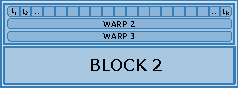
\includegraphics[scale=2]{figures/gpu_threads.pdf}
    \centering
    \caption{GPU thread hierarchy. A block consists of a number warps, all of which has a fixed number of threads (32 on modern NVIDIA hardware \citep{nvidiaadaarch}), besides the last which might have fewer.}
\end{figure}

CUDA (Compute Unified Device Architecture) has been the dominant programming model for utilising GPUs for general-purpose computations. CUDA allow kernels to be written in C++. Kernels refer to GPU programs that run in parallel. Kernels have limited options for synchronising between threads during execution. Therefore, algorithms typically consist of multiple kernels being dispatched from the CPU. To write high-performance kernels, a few factors have to be kept in mind. Note that we specifically refer to the architecture of modern NVIDIA GPUs, however, similar concepts hold true for other architectures.

\subsection{Thread Occupancy}
Thread occupancy refers to the percentage of the maximum possible warps being active at any given time. On NVIDIA GPUs, occupancy is typically measured per SM (Streaming Multiprocessor). Each SM can execute a limited amount of blocks and warps concurrently. If a subset of warps within a block takes longer to complete than the rest, it prevents new blocks from launching. Similarly, if a subset of blocks takes longer than the rest, it blocks the kernel from finishing. Besides leaving cores unused, it also makes the running cores less efficient as SIMD units have fewer warps to interleave. It is therefore crucial to balance work across warps and blocks \citep{Jeon2022}.

\subsection{Memory Access}
Memory access patterns can have a large impact on the performance of kernels. Because warps execute in a SIMD fashion, whenever data is accessed, the whole warp has to wait until the data has been fetched for all threads. It is therefore beneficial for warps to fetch data consecutive in memory. Because the L1 cache is local to each SM, it is also beneficial for threads within a block to access data close in memory.\\

Modern GPUs are prone to memory bandwidth bottlenecks. This means that situations occur where all warps managed by a SIMD unit are stalled because of memory reads. For this reason, it can at times be beneficial to use techniques such as \textit{recomputation} and \textit{kernel fusion}. \textit{Recomputation} attempts to lower the amount of memory accessed by recomputing results instead of fetching them from memory. This shifts more load to the ALU (Arithmetic Logic Unit), which may otherwise be idle. \textit{Kernel fusion} attempts the same by avoiding loads and stores by merging consecutive kernels and keeping the data in registers.

\begin{figure}[h]
    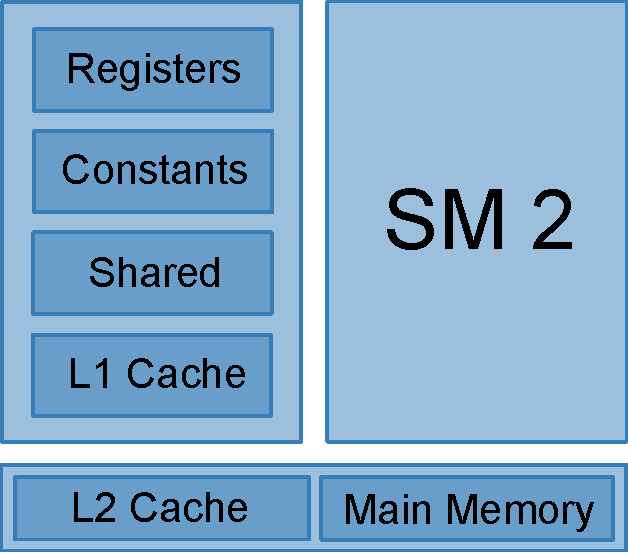
\includegraphics[scale=0.5]{figures/gpu_memory.pdf}
    \centering
    \caption{GPU memory hierarchy. SMs share registers, constants, shared memory and L1 cache, whereas L2 cache and memory is shared between SMs. Generally, memory is accessed fastest in registers and slowest in main memory \citep{nvidiaadaarch}.}
    \label{gpu_memory}
\end{figure}

As illustrated in Figure \ref{gpu_memory}, registers are shared between all warps in a SM unit. This means that the amount of registers used by a kernel can limit the amount of warps that can run in parallel.

\subsection{Divergence}
Because all threads of a warp execute in lockstep, branching can lead to performance problems if the threads diverge. If a branch is taken by a subset of threads in a warp, the whole warp waits until those threads are done executing the branch. It is therefore beneficial to assign work to threads such that all threads of a warp take similar branches.

\subsection{Floating Point Formats}\label{float_speed}
Modern GPU architectures are optimized for 32-bit and 16-bit floats. NVIDIA report 64 times fewer 64-bit float FLOPS (Floating Point Operations Per Second) compared to 32-bit floats on their ADA architecture \citep{nvidiaadaarch}.
It is therefore advantageous to do as many operations as possible with 32-bit floats.



\section{cuGAL}
We now describe the different stages of the cuGAL algorithm in detail.

\subsection{Sinkhorn-Knopp}
As mentioned in Section \ref{float_speed}, modern GPUs are optimised for 32-bit floats. This poses a challenge for Sinkhorn-Knopp, which is prone to overflows. Using 32-bit floats results in overflows at values exceeding $3.4 \times 10^{38}$ \citep{ieeefloat}. In the Sinkhorn-Knopp algorithm, we perform computations of the form $e^{-x}$. This means that if $A$ contains entries below approximately $-88.72$ an overflow will occur, as $3.4 \times 10^{38} \lesssim e^{-88.72}$. A solution to this problem is doing all calculations in the log-domain. Performing Sinkhorn-Knopp iterations in the log domain is not a new technique, and has before been used to avoid issues arising from numerical instability \citep{chizat2017sinkhornlog}. %although to the best of our knowledge, no specific publication first introduced this adaptation of the Sinkhorn-Knopp algorithm.

\subsubsection{Log-Variant}
\begin{algorithm}[H]
\caption{Sinkhorn-Knopp-log}\label{alg:sinkhorn_log}
\textbf{Input:} $A \in \mathds{R}^{n \times n}, a, b \in \mathds{R}^{n}, \epsilon \in \mathds{R}$
\begin{algorithmic}[1]
\State $K \gets -A / \epsilon$
\State $a, b \gets \log(a), \log(b)$
\State $u \gets \text{initial guess, see Section \ref{warm-start}}$
\For{$i \gets 1, .., \text{it}$}
    \State $v \gets b - \texttt{logsumexp}(K + \begin{bmatrix} u & .. & u \end{bmatrix})$ \Comment{For each row}
    \State $u \gets a - \texttt{logsumexp}(K^T + \begin{bmatrix} v & .. & v \end{bmatrix})$ \Comment{For each row}
    \If {stop condition met}
        \State \textbf{break}
    \EndIf
\EndFor
\State \Return $\exp(K + \begin{bmatrix} u & .. & u \end{bmatrix} + \begin{bmatrix} v & .. & v \end{bmatrix}^T)$
\end{algorithmic}
\end{algorithm}

\texttt{logsumexp} is defined as:
\begin{equation}
    \begin{split}
        \texttt{logsumexp}(x) = \log(\sum_{i = 1}^n e^{x_i}) = \log(\sum_{i = 1}^n e^a e^{x_i - a}) = \log(e^a \sum_{i = 1}^ne^{x_i - a}) = a +\log(\sum_{i = 1}^ne^{x_i - a})
    \end{split}
\end{equation}

$a$ can be defined as $a = \max(x)$, which ensures that the largest exponent calculated is $\exp(0) = 1$. \\

We provide an efficient CUDA implementation of Sinkhorn-Knopp-log using \textit{kernel fusion}. We specifically avoid writing the results of $K + \begin{bmatrix} u & .. & u \end{bmatrix}$ and $K^T + \begin{bmatrix} v & .. & v \end{bmatrix}$ to memory by performing each scaling operation in a single fused kernel.

We assign a thread block in CUDA to calculate \texttt{logsumexp} across the rows of $A$ in parallel. We realise that because peak memory usage is used calculating the gradient, we can store the transpose of $A$ in memory without increasing memory requirements. This allows us to only have blocks collaborate across rows, which leads to favourable memory access patterns as we store all matrices as row-major layout. For further details, see CUDA source code in Appendix \ref{sinkhorn_log_impl}.

\subsubsection{Mix-Variant}
For large graphs, Sinkhorn-Knopp-log can be slow as a result of performing the $O(n^2)$ $\exp$ operations each iteration requires, which is significantly more ALU (Arithmetic Logical Unit) intensive compared to operations such as multiplication and addition.

We provide a simple, and as far as we are aware, novel solution that avoids overflows for 32-bit integers with precision close to Sinkhorn-Knopp-log in many cases. We call this method Sinkhorn-Knopp-mix, as it performs a single row scaling in the log domain before continuing using the classic Sinkhorn-Knopp algorithm.

\begin{algorithm}[H]
\caption{Sinkhorn-Knopp-mix}\label{alg:sinkhorn_mix}
\textbf{Input:} $A \in \mathds{R}^{n \times n}, a, b \in \mathds{R}^{n}, \epsilon \in \mathds{R}$
\begin{algorithmic}[1]
\State $K \gets -A / \epsilon$
\State $v \gets \log(b) - \texttt{logsumexp}(K)$
\State $K \gets \exp(K + \begin{bmatrix} v & .. & v \end{bmatrix}^T)$
\State $u \gets \text{initial guess, see Section \ref{warm-start}}$
\For{$i \gets 1, .., \text{it}$}
    \State $v \gets \frac{b}{uK}$
    \State $u \gets \frac{a}{Kv}$
    \If {stop condition met}
        \State \textbf{break}
    \EndIf
\EndFor

\State \Return $\text{diag}(u)K\text{diag}(v)$

\end{algorithmic}
\end{algorithm}

\subsubsection{Warm Start}\label{warm-start}
Choosing an initial $u$ scaling vector is crucial for reducing the number of iterations Sinkhorn-Knopp requires to converge. The standard choice of initialising all entries with $1/n$ is sub optimal. We find that the simple choice of using the resulting $u$ from the previous Frank-Wolfe iteration works very well in most cases, especially when the amount of noise is low.
\pgfplotstableread[col sep=comma]{data/sums.csv}\cache
\begin{figure}[H]
    \centering
    \begin{tikzpicture}
        \begin{axis}[
            width=\linewidth*0.5,
            xlabel={Noise},
            ylabel={Time (s)},
            xtick=data,
            xticklabels = {0.00, 0.05, 0.10, 0.15, 0.20, 0.25},
            legend pos=south west,
            legend style={at={(0.5,-0.20)}, anchor=north, legend columns=-1, font=\small},
            ymajorgrids=true,
            xmajorgrids=true,
        ]
        \addplot table[x index=\coordindex, y index=1] {\cache};
        \addplot table[x index=\coordindex, y index=2] {\cache};
        \legend{initialise with $1/n$, initialise with previous $u$}
        \end{axis}
    \end{tikzpicture}
    \caption{Running time of \textsc{cuGAL} with Sinkhorn-Knopp-mix \ref{alg:sinkhorn_mix} (MIX) with and without the warm start described in Section \ref{warm-start} on bio-dmela with varying levels of noise.}
    \label{fig:SK_accu}
\end{figure}


\subsubsection{Stop Condition}
The most traditional choice of stopping condition is checking whether the sums of the columns and rows of $\text{diag}(u)K\text{diag}(v)$ has converged close to $a$ and $b$. Instead, we choose to stop when the scaling vectors $u$ and $v$ have converged to a stable point. We take inspiration from \cite{li2023importance}, where the absolute difference between the scaling vectors from the previous iteration is considered. We specifically use the following condition for some vector $a$ and threshold $\delta$:
\begin{equation}
    \frac{\max(|a^{(i)} - a^{(i - 1)}|)}{\max(\max(|a|), \max(|a^{(i - 1)}|))} < \delta
\end{equation}

We use a relative difference to better adapt to cost matrices with high entries. The difference compared to the more traditional choice of checking for convergence mainly has to do with numeric stability. We observe that using 32-bit floats can halt the rate of convergence in certain numerically tricky situations. Checking only $u$ and $v$ also has the advantage of being faster, making it less computationally expensive to check for convergence.

If $\delta$ is chosen to be too high, Sinkhorn-Knopp will exit before properly converging which will cause a drop in accuracy. On the other hand, choosing a $\delta$ too small, will result in many redundant iterations. We find that determining a general set point where the threshold begins to hurt accuracy is challenging. Testing certain experiments with varying thresholds, we observe very significant drops in accuracy for higher thresholds, while for others, we observe almost no drop to accuracy. This can be the case on similar datasets, using similar settings. Anecdotally, we observe that the mix-variant responds worse to higher values than the log-variant. In Figure \ref{fig:SK_accu}, we see an example of this inconsistency, where even for very high $\delta$s, accuracy seems high, until it suddenly drops. 

\pgfplotstableread[col sep=comma]{data/sink_thres_bd_accu.csv}\sinkthresbdaccu
\begin{figure}[H]
    \centering
    %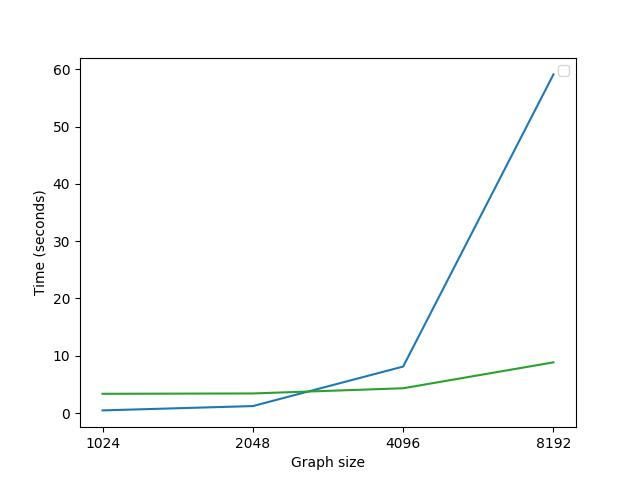
\includegraphics[width=\textwidth]{figures/sparse_vs_normal_gradient_time.jpg}
    \begin{tikzpicture}
        \begin{axis}[
            width=\linewidth*0.5,
            xlabel={Noise},
            ylabel={Accuraccy},
            x dir=reverse,
            legend pos=south west,
            xtick=data,
            xticklabels={$0.0$, $0.1$, $0.2$, $0.3$, $0.4$, $0.5$},
            %yticklabel={\pgfmathprintnumber[fixed,precision=2]{\tick}},
            legend style={at={(0.5,-0.20)}, anchor=north, legend columns=4, font=\small},
            ymajorgrids=true,
            xmajorgrids=true,
        ]
        \pgfplotsforeachungrouped \i in {0, 1, 2, 3, 4, 5, 6, 7} {
            \addplot table[x index=0, y expr=\thisrowno{\i}] 
            {\sinkthresbdaccu};
            }
        \legend{\textsc{LOG} $\delta = 0.1$, \textsc{LOG} $\delta = 0.3$, \textsc{LOG} $\delta = 0.5$, \textsc{LOG} $\delta = 1.0$,\textsc{MIX} $\delta = 0.1$, \textsc{MIX} $\delta = 0.3$, \textsc{MIX} $\delta = 0.5$, \textsc{MIX} $\delta = 1.0$}
        \end{axis}
    \end{tikzpicture}
    \caption{Accuracy of different levels of Sinhorn-Knopp threshold using \textsc{cuGAL} with Sinkhorn-Knopp-mix \ref{alg:sinkhorn_mix} (MIX) and \textsc{cuGAL} with Sinkhorn-Knopp-log \ref{alg:sinkhorn_log} (LOG) running on bio-dmela with varying levels of noise.}
    \label{fig:SK_accu}
\end{figure}

We make use of the same regularisation parameter $\epsilon$ and max iteration count $it$ as the implementation given by \cite{fugal2024}, namely $\epsilon = 1$ and $it = 300$.

\subsection{Gradient}
\subsubsection{Sparse Adjacency Matrices}
Working directly with dense adjacency matrices can be memory intensive as each instance requires $O(n^2)$ memory. To exploit the usual sparsity of adjacency matrices, we represent $A$ and $B$ using sparse matrix representations.\\

We use the popular representation CSR (Compressed Sparse Row) \citep{tinney1967csr}. For some $M \in \mathds{R}^{n \times n}$, the CSR representation consists of three vectors: $(C, R, V)$. $|C| = |V| = nnz(M)$, $|R| = n$ where $nnz(M)$ is the number non-zero entries in $M$. $C$ contains column indices of all non-zero entries in each row, starting from row 0. $R$ defines offset into $C$ where each row begins. $V$ contains the value of each non-zero element in the matrix. Because we only represent adjacency matrices of the form $\{0, 1\}^{n \times n}$, we can omit the $V$ vector.\\

CSR representation is especially well suited for matrix multiplications of the form $S \cdot D$, where $S$ is represented using CSR and $D$ is dense.

If we rewrite:
\begin{equation}
    \begin{split}
    \nabla f(P) &= -APB^T - A^TPB + \mu \cdot D\\
    &= (B^T(-A^TP)^T)^T - (B(AP)^T)^T + \mu \cdot D
    \end{split}
\end{equation}

the gradient can be calculated using only matrix multiplication of the form $S \cdot D$. This requires $A^T$ and $B^T$ to either be recalculated in each iteration or stored explicitly. If the graphs are undirected, we can exploit the fact that $A = A^T$ and $B = B^T$:
\begin{equation}
    \begin{split}
    \nabla f(x) &= (B(-AP)^T)^T - (B(AP)^T)^T + \mu \cdot D\\
    &= -2 \cdot (B (A P)^T)^T + \mu \cdot D
    \end{split}
\end{equation}

which halves the number of matrix multiplications required.

\subsubsection{Implementation}
We utilize \textit{recomputation} to avoid storing the distance matrix $D$. We instead use a custom kernel to recompute the Euclidean distances from Equation \ref{euclidean_distance_matrix} each time we compute $f(x)$. This both speeds up the computation and lowers the amount of $n \times n$ matrices required in memory by one. In addition, we use \textit{kernel-fusion} to speed up the computation of $g(x)$ by merging it with the kernel for computing $f(x)$, which avoids storing and loading intermediate results.

\begin{algorithm}[H]
\caption{sparse-calculate-gradient}\label{alg:cugal-calculate-gradient}
\textbf{Input:} $\lambda \in \mathds{R}$
\textbf{Input:} $Q \in \mathds{R}^{n \times n}$
\begin{algorithmic}[1]
\State $X \gets (B (A P)^T)^T$ \Comment{Using sparse matrix multiplication}

\For{$i, j \gets 1 \textbf{ to } \text{n}$} \Comment{In parallel}
    \State $a \gets \text{Euclidean-distance}((F_1)_{i,:}, (F_2)_{j:})$
    \State $r \gets 1 - 2Q_{i, j}$
    \State $X_{i, j} \gets -2 X_{i, j} + \mu a + \lambda r$
\EndFor

\State \Return $X$
\end{algorithmic}
\end{algorithm}

In addition, we also construct the sparse matrix representations directly from edge lists of the form $E \in (\mathds{Z_+}, \mathds{Z_+})^m$ on the GPU.

\begin{algorithm}[H]
\caption{construct-adjacency}
\textbf{Input:} $E \in (\mathds{Z_+}, \mathds{Z_+})^m$
\begin{algorithmic}[1]
    \State $E \gets$ radix-sort($E$) \Comment{Sort first by row then by column}
    \State $C, R \gets \vec{0}, \vec{0}$
    \For{$i \gets 1 \textbf{ to } |E| - 1$} \Comment{In parallel}
        \State $(a, \_), (b, \_) \gets E_i, E_{i + 1}$
        \State $b \gets E_{i + 1}$
        \For{$j \gets a + 1 \textbf{ to } b$}
            \State $R_j \gets i + 1$
        \EndFor
    \EndFor
    \For {$i \gets 1 \textbf{ to } |E| - 1$} \Comment{In parallel}
        \State $(\_, c) \gets E_i$
        \State $C_i \gets c$
    \EndFor
    \State \Return $C, R$
\end{algorithmic}
\end{algorithm}

\subsubsection{Performance}
\pgfplotstableread[col sep=comma]{data/memory_usage.csv}\mem

\begin{figure}[H]
    \centering
\begin{tikzpicture}
\begin{axis}[
    ymin=0,
    xtick=data,
    xticklabels={$2^8$, $2^9$, $2^{10}$, $2^{11}$, $2^{12}$, $2^{13}$, $2^{11}$, $2^{12}$},
    legend style={at={(0.285, 1)}, anchor=north, legend columns=1},
    bar width=12pt,
    width=\textwidth*0.5,
    xlabel={Graph size},
    ylabel={Peak memory usage in bytes},
    ymajorgrids=true,
    xmajorgrids=true,
]
\addplot table[x expr=\coordindex, y index=0] {\mem};
\addplot table[x expr=\coordindex, y index=1] {\mem};
\addplot table[x expr=\coordindex, y index=2] {\mem};
\legend{\textsc{Fugal}, \textsc{cuGAL} dense, \textsc{cuGAL} sparse}
\end{axis}
\end{tikzpicture}
    \caption{Scaling of peak memory usage of \textsc{Fugal} and \textsc{cuGAL} on NW graphs with parameters $k=7, p=0.1$ and no noise.}
    \label{fig:fugal-scaling}
\end{figure}

\begin{figure}[H]
    \centering
    %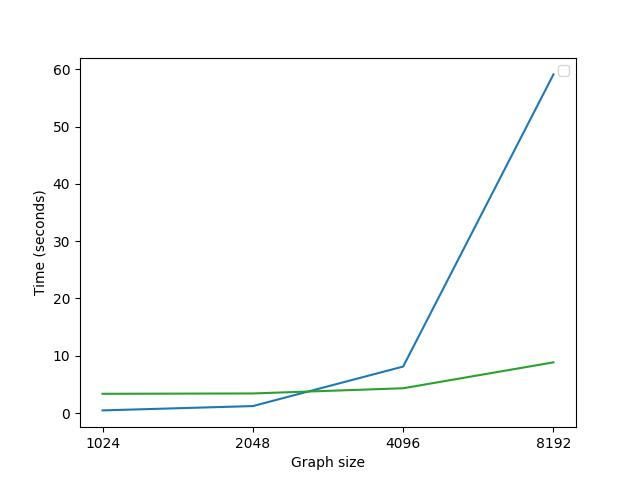
\includegraphics[width=\textwidth]{figures/sparse_vs_normal_gradient_time.jpg}
    \begin{tikzpicture}
        \begin{axis}[
            xlabel={Graph size},
            ylabel={Time (s)},
            ymajorgrids=true,
            xmajorgrids=true,
            xtick={1024, 2048, 4096, 8092},
            xticklabels={$2^{11}$, $2^{12}$, $2^{13}$, $2^{14}$},
            legend style={at={(0.7, 1)}, font=\small},
            width=\textwidth*0.5,
        ]
        \addplot table {data/dense_gradient_NSW_k10_p05.dat};
        \addplot table {data/sparse_gradient_NSW_k10_p05.dat};
        \legend{Dense (Algorithm \ref{alg:calculate-gradient}), Sparse (Algorithm \ref{alg:cugal-calculate-gradient})}
        \end{axis}
    \end{tikzpicture}
    \caption{Time spent calculating gradient for NW graphs with parameters $k=10$, $p=0.5$.}
    \label{fig:sparse_speed}
\end{figure}

Figure \ref{fig:sparse_speed} portrays the performance of using the sparse matrix multiplication for the calculating the gradient for Newmann-Watts graphs with node degree $k = 10$ and rewrite probability $p = 0.5$. While using dense adjacency matrices show better performance for smaller graphs, we observe better scaling of sparse matrix multiplication for larger graphs.

From Figure \ref{fig:fugal-scaling} we observe a significant decrease in memory from using sparse adjacency matrices. Along with more inline operations and using 32-bit floats instead of 64-bit floats, we also observe significantly lower memory usage compared to \textsc{Fugal}.

\subsection{Feature Extraction}
Feature extraction has a computational cost of $O(nM^2)$ where $M$ is the maximum degree of any vertex \citep{fugal2024}. As observed, this takes up a minor part of the overall runtime of \textsc{Fugal} (Figure \ref{fig:fugal-scaling}). However, we observe that as we optimise the rest of the algorithm, feature extraction can take up a significant part of runtime for large graphs. We therefore implement an optimised GPU implementation of feature extraction.\\

To avoid the memory cost of dense adjacency matrices, we work directly with CSR-compressed representations. 

\begin{algorithm}[H]
\caption{vertex-features}\label{alg:cugal-vertex-features}
\textbf{Input:} $(C, R, V)$ \Comment{CSR compressed matrix.}
\begin{algorithmic}[1]
\State $D \gets \vec{0}, C \gets \vec{0}$ \Comment{Vertex degrees and clustering coefficients}
\For{$i \gets 1, .., \text{n}$} \Comment{In parallel}
    \For{$j \gets R_i \textbf{ to } R_{i + 1}$} \Comment{For every neighbor}
        \State $A \gets \{ C_k | k \in R_i, .., R_{i + 1} \}$
        \State $B \gets \{ C_k | k \in R_j, .., R_{j + 1} \}$
        \State $C_i \gets C_i + |A \cap B|$
    \EndFor
    \State $D_i \gets R_{i + 1} - R_i$
\EndFor
\State \Return $D$, $C$
\end{algorithmic}
\end{algorithm}

Because the column indices of $C$ are sorted, the intersection size can be found in linear time without additional memory. Finding the average features of neighbours is done in a similar fashion.\\

We acknowledge that even more optimised implementations are possible, as our implementation can experience occupancy issues for graphs where the degree of nodes varies a lot across nodes. We restrain from further optimisations, as our implementation sufficiently improves the performance of feature extraction to make it an insignificant part of the overall runtime.

\subsection{Frank-Wolfe}
\textsc{FUGAL} performs a fixed amount of Frank-Wolfe iterations. However, we observe that the number of iterations required to converge varies depending on the graph and noise level. We define a threshold $\gamma$ on the change to $Q$ which allows us to stop early in certain cases. The threshold must not be too large, as this has two adverse effects. Firstly, the Hungarian algorithm requires more iterations to find the optimal assignment, and secondly, if the resulting difference is too large, some assignments might differ and decrease accuracy. To find a fitting threshold, we run experiments on real datasets with varying levels of synthetic noise.\\

\pgfplotstableread[col sep=comma]{data/fw_thresh_bio-dmela.csv}\fwtbm
\pgfplotstableread[col sep=comma]{data/fw_thres_bd_times.csv}\fwtbmt
\begin{figure}[H]
    \centering
    %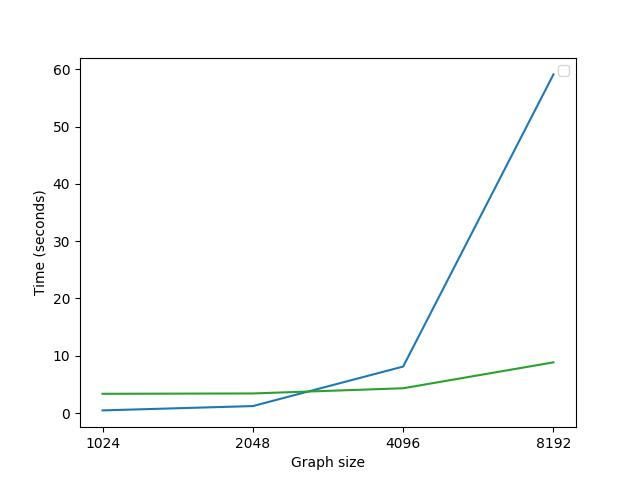
\includegraphics[width=\textwidth]{figures/sparse_vs_normal_gradient_time.jpg}
    \begin{tikzpicture}
        \begin{axis}[
            width=\linewidth*0.5,
            xlabel={Noise},
            ylabel={Accuraccy},
            x dir=reverse,
            legend pos=south west,
            xtick=data,
            xticklabels={$0.0$, $0.1$, $0.2$, $0.3$, $0.4$, $0.5$},
            %yticklabel={\pgfmathprintnumber[fixed,precision=2]{\tick}},
            legend style={at={(0.5,-0.20)}, anchor=north, legend columns=3,},
            ymajorgrids=true,
            xmajorgrids=true,
        ]
        \pgfplotsforeachungrouped \i in {1,2,3,4,5,6} {
            \addplot table[x index=0, y expr=\thisrowno{\i}] 
            {\fwtbm};
            }
        \legend{$\gamma = 0.00$, $\gamma = 0.05$, $\gamma = 0.10$, $\gamma = 0.20$, $\gamma = 0.50$, $\gamma = 1.00$}
        \end{axis}
    \end{tikzpicture}
    \caption{Accuracy of different levels of $\gamma$. \textsc{cuGAL} with Sinkhorn-Knopp-mix \ref{alg:sinkhorn_mix} on bio-dmela}
    \label{fig:FW_accu}
\end{figure}
\hfill
\begin{figure}[H]
    \begin{tikzpicture}
        \begin{semilogyaxis}[
                width=\linewidth,
                ybar stacked,
                log origin=infty,
                ylabel={Time $(s)$},
                xlabel={Noise},
                x label style={at={(0.5, -0.07)}},
                bar width=6pt,
                legend pos=south west,
                xtick=\empty,%{3.5, 10.5, 17.5, 24.5, 31.5, 38.5},
                %xticklabels={0, 5, 10, 15, 20, 25},
                %x tick label style={\empty}
                %extra x tick style={xshift=,},
                legend style={at={(0.5,-0.12)}, anchor=north, legend columns=-1},
                %yticklabel={\pgfmathprintnumber[fixed,precision=2]{\tick}},
                ymajorgrids=true,
                xmajorgrids=true,
            ]
            \pgfplotsforeachungrouped \i in {0,1,2,3} {
                    \addplot table[x expr=\coordindex, y index=\i]
                        {\fwtbmt};
                }

            %\legend{$ \displaystyle { \text{Sinkhorn-} \atop \text{Knopp} }$, $ \displaystyle { \text{Feature} \atop \text{Extraction} }$, Gradient, Hungarian};
            \legend{Sinkhorn-Knopp-mix \ref{alg:sinkhorn_mix}, Feature Extraction, Gradient \ref{alg:cugal-calculate-gradient}, Hungarian};
            \coordinate (brace1start) at (axis cs:00.5,19e-2);
            \coordinate (brace1end)   at (axis cs:07.5,19e-2);
            \coordinate (brace2end)   at (axis cs:14.5,19e-2);
            \coordinate (brace3end)   at (axis cs:21.5,19e-2);
            \coordinate (brace4end)   at (axis cs:28.5,19e-2);
            \coordinate (brace5end)   at (axis cs:35.5,19e-2);
            \coordinate (brace6end)   at (axis cs:42.5,19e-2);

        \end{semilogyaxis}
        % Adding the braces
        \draw [decorate,decoration={brace,amplitude=10pt,mirror,raise=4ex}]
        (brace1start) -- (brace1end) node[midway,yshift=-3.5em]{0};
        \draw [decorate,decoration={brace,amplitude=10pt,mirror,raise=4ex}]
        (brace1end) -- (brace2end) node[midway,yshift=-3.5em]{5};
        \draw [decorate,decoration={brace,amplitude=10pt,mirror,raise=4ex}]
        (brace2end) -- (brace3end) node[midway,yshift=-3.5em]{10};
        \draw [decorate,decoration={brace,amplitude=10pt,mirror,raise=4ex}]
        (brace3end) -- (brace4end) node[midway,yshift=-3.5em]{15};
        \draw [decorate,decoration={brace,amplitude=10pt,mirror,raise=4ex}]
        (brace4end) -- (brace5end) node[midway,yshift=-3.5em]{20};
        \draw [decorate,decoration={brace,amplitude=10pt,mirror,raise=4ex}]
        (brace5end) -- (brace6end) node[midway,yshift=-3.5em]{25};

    \end{tikzpicture}
    \caption{Speed of different levels of $\gamma$. There are six levels of increasing noise, each tested with six increasing $\gamma$ thresholds.}
    \label{fig:FW_speed}
\end{figure}

Figure \ref{fig:FW_speed} shows how, as the threshold rises, the accumulated time spent running Sinkhorn-Knopp and computing the gradient decreases. Here we observe, that when the noise increases and when the Frank-Wolfe algorithm converges less, the Hungarian algorithm uses more time to find an optimal assignment. Figure \ref{fig:FW_accu} shows the effect of the threshold on the accuracy. For small thresholds, the accuracy is unaffected as either no iterations are skipped, or the resulting \textit{quasi-permutation} matrix is similar enough for the Hungarian algorithm to round to the same answer. For larger thresholds, we see a gradual effect on accuracy, which must be weighed against the speedup for each application of the algorithm. 

\pgfplotstableread[col sep=comma]{data/fw_thres_bd_time_per_accu_thres_noise.csv}\fwbdtptn

\iffalse
\begin{figure}
    \centering
    \begin{tikzpicture}
    \begin{axis}[
        xlabel={X axis label}, % Replace with your x-axis label
        ylabel={Y axis label}, % Replace with your y-axis label
        legend style={at={(1.05,1)}, anchor=north west},
        scatter/classes={
            0.00_0.00={mark=square*,blue},
            0.00_0.01={mark=square*,red},
            0.00_0.05={mark=square*,black},
            0.01_0.00={mark=triangle*,blue},
            0.01_0.01={mark=triangle*,red},
            0.01_0.05={mark=triangle*,black},
            0.05_0.00={mark=o,blue},
            0.05_0.01={mark=o,red},
            0.05_0.05={mark=o,black}
        }
    ]
        \addplot[
            scatter,
            only marks,
            point meta=explicit symbolic,
            visualization depends on={value \thisrow{meta} \as \class},
            scatter src=explicit symbolic
        ] table[x index=0, y index=1, meta expr={\thisrow{shape} _ \thisrow{color}}] {\fwbdtptn};
    \end{axis}
    \end{tikzpicture}
    \caption{Caption}
    \label{fig:enter-label}
\end{figure}
\fi

\subsection{Hungarian}
To round to a permutation matrix, \textsc{Fugal} uses the Hungarian Algorithm. We observe that Frank-Wolfe in almost all cases converges to a shape very close to a permutation matrix. To take advantage of this, we experiment with a greedy LAP approximator. We find an assignment by greedily choosing the unassigned row and column with the highest entry, the algorithm works well for permutation-like matrices.\\

\begin{algorithm}[H]
\caption{greedy-lap}\label{alg:greedy-lap}
    \textbf{Input:} $Q \in R^{n \times n}$
    \begin{algorithmic}
        \State $M \in R^n \gets \boldsymbol{1}$     \Comment{A mask that keeps track of used columns}
        \State $I \in R^n \gets \boldsymbol{0}$ \Comment{Indices of columns in permutation matrix}
        \State $Q \gets$ sort-rows-by-max-value$(Q)$
        \For{$row \in Q$}
            \State $row \gets row\times M$ \Comment{Values in columns already used are set to 0}
            \State $col \gets$ max$(row)$
            \State $I_{row} \gets col$
            \State $M_{col} \gets 0$
        \EndFor
        \State \Return $I$
    \end{algorithmic}
\end{algorithm}

This allows us to round to a permutation matrix in $O(n^2)$ compared to the $O(n^3)$ of the Hungarian algorithm.\\

% We can now prove that for all rows with a max entry above a threshold, the greedy algorithm will pick the same assignment as the optimal solution. We keep track of two sums, $A$ and $B$. $A$ is the sum of all entries chosen by the assignment, while $B$ is all entries excluded by the previous assignments, meaning all other entries in the assigned rows and columns. When the algorithm picks an entry $(i, j)$ for the assignment, $A \gets A + C_{i, j}$, while $B \gets B + 2(1 - C_{i, j})$. This implies that if $C_{i, j} > 2(1 - C_{i, j}) = C_{i, j} > \frac{2}{3}$ then all other assignments including the same row or column will be worse.\\

Empirically, we find that greedy-lap (Algorithm \ref{alg:greedy-lap}) usually achieves the same or very similar results to the Hungarian algorithm for experiments with low amounts of noise (Figure \ref{fig:greedy-accu}).

\pgfplotstableread[col sep=comma]{data/more_greedy_vs_scipy_wFW20_enron_accu.csv}\mgsea
\begin{figure}[H]
    \centering
    \begin{tikzpicture}
        \begin{axis}[
            xmajorgrids=true, ymajorgrids=true,
            xlabel={Noise}, ylabel={Accuracy},
            xtick=data,
            xticklabels={0.0, 0.1, 0.2, 0.3},
            legend style={legend cell align={left}}
        ]
            \addplot table[ x expr=\coordindex, y index=0 ] {\mgsea};
            \addplot table[ x expr=\coordindex, y index=1 ] {\mgsea};
            \addplot table[ x expr=\coordindex, y index=2 ] {\mgsea};
            \addplot table[ x expr=\coordindex, y index=3 ] {\mgsea};
            \legend{Hungarian, Hungarian with $\gamma=0.2$, Greedy, Greedy with $\gamma=0.2$}
        \end{axis}
    \end{tikzpicture}
    \caption{\textsc{cuGAL} with Sinkhorn-Knopp-mix (Algorithm \ref{alg:sinkhorn_mix}) on email-Enron with varying levels of noise, demonstrating the difference between using the Hungarian algorithm and our greedy approximation.}
    \label{fig:greedy-accu}
\end{figure}

\pgfplotstableread[col sep=comma]{data/more_greedy_vs_scipy_wFW20_enron.csv}\mgse
\begin{figure}[H]
\centering
\begin{tikzpicture}
% Plot the axis
\begin{axis}[
    ybar stacked,
    ymin=0,
    xtick=data,
    xticklabels={A, B, C, D, A, B, C, D, A, B, C, D, A, B, C, D},
    legend style={at={(0.5,-0.15)}, anchor=north, legend columns=4},
    bar width=12pt,
    width=\textwidth,
    height=\textwidth,
    xlabel={Graph size},
    x label style={at={(0.5, -0.1)}},
    ylabel={Time in seconds},
    ymajorgrids=true,
    xmajorgrids=true,
    clip=false % To allow drawing outside the axis
]

\addplot table[x expr=\coordindex, y index=0] {\mgse};
\addplot table[x expr=\coordindex, y index=1] {\mgse};
\addplot table[x expr=\coordindex, y index=2] {\mgse};
\addplot table[x expr=\coordindex, y index=3] {\mgse};
\legend{Sinkhorn-Knopp, Feature Extraction, Gradient, Hungarian};

% Define coordinates for braces
\coordinate (brace1start) at (axis cs:0.5,10);
\coordinate (brace1end) at (axis cs:4.5,10);
\coordinate (brace2start) at (axis cs:4.5,10);
\coordinate (brace2end) at (axis cs:8.5,10);
\coordinate (brace3start) at (axis cs:8.5,10);
\coordinate (brace3end) at (axis cs:12.5,10);
\coordinate (brace4start) at (axis cs:12.5,10);
\coordinate (brace4end) at (axis cs:16.5,10);

% Define coordinate for the legend node
\coordinate (legendpos) at (axis cs:8.5, -150);

\end{axis}

% Adding the braces
\draw [decorate,decoration={brace,amplitude=10pt,mirror,raise=4ex}]
(brace1start) -- (brace1end) node[midway,yshift=-3em]{0.0 noise};
\draw [decorate,decoration={brace,amplitude=10pt,mirror,raise=4ex}]
(brace2start) -- (brace2end) node[midway,yshift=-3em]{0.1 noise};
\draw [decorate,decoration={brace,amplitude=10pt,mirror,raise=4ex}]
(brace3start) -- (brace3end) node[midway,yshift=-3em]{0.2 noise};
\draw [decorate,decoration={brace,amplitude=10pt,mirror,raise=4ex}]
(brace4start) -- (brace4end) node[midway,yshift=-3em]{0.3 noise};
        
% Adding the legend node
\node[draw] at (legendpos) {A: Hungarian\quad B: Hungarian with $\gamma=0.2$\quad C: Greedy\quad D: Greedy with $\gamma=0.2$};

\end{tikzpicture}
\caption{\textsc{cuGAL} with Sinkhorn-Knopp-mix (Algorithm \ref{alg:sinkhorn_mix}) with Frank-Wolfe threshold of $\gamma = 0$ and $\gamma=0.2$, at different levels of noise. The graph is email-Enron.}
\label{fig:hungarian-scipy-greedy}
\end{figure}

Figure \ref{fig:hungarian-scipy-greedy} shows the possible performance improvements of using our greedy approximator over the Hungarian algorithm.

\subsection{The \textsc{cuGAL} Algorithm}
We now derive the full \textsc{cuGAL} algorithm.

\begin{algorithm}[H]
\caption{cuGAL}\label{alg:cugal-vertex-features}
\textbf{Input:} $G_1, G_2$ \Comment{Input graphs}\\
\textbf{Input:} $T, \mu, \delta, \gamma$
\begin{algorithmic}[1]
    \State $A, B \gets \text{construct-adjacency}(G_1), \text{construct-adjacency}(G_2)$
    \State $F_1, F_2 \gets \text{extract-features}(A), \text{extract-features}(B)$
    \State $Q \gets \boldsymbol{1} \cdot \boldsymbol{1}^T / n$
    \For{$\lambda = 0$ \textbf{to} $T - 1$}
        \For{$it = 1$ \textbf{to} $10$} \Comment{Do 10 Frank-Wolfe iterations}
            \State $grad \gets \text{sparse-calculate-gradient}(Q, \lambda)$
            \State $q_{it} \gets \text{Sinkhorn-Knopp-\{mix, log\}}(\boldsymbol{1}, \boldsymbol{1}, grad)$
            \State $\alpha \gets \frac{2}{2 + it}$
            \State $\Delta \gets \alpha(q_{it} - Q)$
            \State $Q \gets Q + \Delta$
            \If {$\text{max}(|\Delta|) < \gamma$}
                \State \textbf{break}
            \EndIf
        \EndFor
    \EndFor
\State \Return $\{\text{hungarian}, \text{greedy-lap}\}(Q)$
\end{algorithmic}
\end{algorithm}

We implement \textsc{cuGAL} in a mixture of PyTorch and CUDA. It is made to be configurable to let the user balance speed and accuracy. In fact, \textsc{cuGAL} can be configured to run as \textsc{Fugal}. This makes \textsc{cuGAL} flexible to handle many different types of graphs and desired levels of accuracy \footnote{Code can be found at: \url{https://github.com/SebastianRueClausen/cuGAL}}. 

Using sparse adjacency matrices for undirected graphs, \textsc{cuGAL} only requires 3 $n \times n$ matrices in memory. This optimisation, combined with the use of 32-bit floats, means that \textsc{cuGAL} can run on significantly larger graphs in the same amount of memory compared to \textsc{Fugal}.

\subsection{Time Complexity of \textsc{cuGAL}}
Using sparse matrix representation and greedy rounding to a permutation matrix, \textsc{cuGAL} improves the theoretical time complexity of \textsc{Fugal}. \cite{fugal2024} shows that \textsc{Fugal} runs in $O(n^3)$. Calculating the gradient (Algorithm \ref{alg:cugal-calculate-gradient}) runs in $O(n^2 + nnz(A) \cdot n + nnz(B) \cdot n)$ compared to $O(n^3)$ in \textsc{Fugal} (Algorithm \ref{alg:calculate-gradient}). Rounding to a permutation matrix (Algorithm \ref{alg:greedy-lap}) is $O(n^2)$ compared to $O(n^3)$ in \textsc{Fugal}. Sinkhorn-Knopp runs in nearly $O(n^2)$ \citep{cuturi2013sinkhorn}, which also is the case for the log and mix variant. The rest of the algorithm runs in $O(n^2)$ or lower. Since at most $10 \cdot T$ Frank-Wolfe iterations are performed, and $T << n$, we do not consider this to contribute to the time complexity.  We therefore conclude that \textsc{cuGAL}, using sparse adjacency matrices and greedy-lap, runs in $O(n^2 + nnz(A) \cdot n + nnz(B) \cdot n)$. In all cases except for fully connected graphs,  $O(n^2 + nnz(A) \cdot n + nnz(B) \cdot n) < O(n^3)$.



\section{Experiments}
To compare our algorithm with \textsc{Fugal}, and verify differences and improvements in speed and accuracy, we run a wide range of benchmarks of graph datasets with both real and synthetic noise. All experiments are performed using the framework presented by \cite{skitsas2023GAEval}. We run all benchmarks of \textsc{cuGAL} on an NVIDIA RTX 3090 GPU, and \textsc{Fugal} on an Intel i9-10940X CPU, using the implementation presented by \cite{fugal2024}.

We run all experiments with the following parameters unless specified otherwise:
\begin{table}[htbp]
    \begin{center}
        \begin{tabular}{ |l|r| }
            \hline
            $\mu$    & $2$     \\
            $\delta$ & $0.001$ \\
            $T$      & $15$    \\
            \hline
        \end{tabular}
    \end{center}
\end{table}

The same $\mu$ and $T$ is used for both \textsc{Fugal} and \textsc{cuGAL}. $\gamma$ is specified for each algorithm, or if not specified, we always run $10$ Frank-Wolfe iterations. We test using both the Hungarian algorithm and our greedy lap approximator (Algorithm \ref{alg:greedy-lap}), with is indicated by \textsc{Greedy}. In addition, we test using both Sinkhorn-Knopp-log (Algorithm \ref{alg:sinkhorn_log}) and Sinkhorn-Knopp-mix (Algorithm \ref{alg:sinkhorn_mix}), which is indicated by \textsc{Log} and \textsc{Mix}. We measure all times as the total wall time for the algorithms to complete. Due to time limitations, only a single run for each algorithm and noise level is performed.

%\subsection{Synthetic graphs}
\subsection{Synthetic noise}
\indent
\resultplot{inf-Power}{data/res_infpow_accu.csv}{data/res_infpow_time.csv}{12}{true}
\resultplot{caGrQc}{data/res_caGrQc_accu.csv}{data/res_caGrQc_time.csv}{12}{false}
\resultplot{erdos}{data/res_erdos_accu.csv}{data/res_erdos_time.csv}{12}{true}
\resultplot{biodmela}{data/res_dmela_oneway_accu.csv}{data/res_dmela_oneway_time.csv}{12}{false}

\resultplot{ca-netscience}{data/res_oneway_canet_accu.csv}{data/res_oneway_canet_time.csv}{12}{true}
\resultplot{Arenas}{data/res_oneway_arenas_accu.csv}{data/res_oneway_arenas_time.csv}{12}{false}
\resultplot{eu-Infroad}{data/res_infroad_accu.csv}{data/res_infroad_time.csv}{12}{true}


\noindent
For graphs with synthetic noise, we test on a selection of large graphs. On bio-dmela with $7 393$ nodes, we see from Figure \ref{fig:biodmela_res} the surprising result that \textsc{cuGAL} achieves higher accuracy than \textsc{Fugal} in all configurations for low amounts of noise. For both no and high amounts of noise, \textsc{Fugal} is competitive with \textsc{cuGAL}, generally ranking between \textsc{cuGAL} with Sinkhorn-Knopp-mix and Sinkhorn-Knopp-log. Similarly on erdos (Figure \ref{fig:erdos_res}), do we observe that \textsc{cuGAL} performs slightly better than \textsc{Fugal} in all cases except for $25\%$ noise. In all other cases does \textsc{Fugal} perform comparable to \textsc{cuGAL} with Sinkhorn-Knopp-log and better than \textsc{cuGAL} with Sinkhorn-Knopp-mix. Using $\gamma = 0.1$ or $\gamma = 0.2$ seems to cause relatively minor decreases to accuracy while providing significant increases in speed. Using greedy rounding varies more. Figure \ref{fig:inf-Power_res} shows a case where greedy rounding causes both significantly lower accuracy and faster performance, indicating that the resulting \textit{quasi-permutation} matrix is a difficult assignment problem for the Hungarian algorithm to solve.


\pgfplotstableread[col sep=comma]{data/res_oneway_caAstroPh_accu_no.csv}\accutable
\pgfplotstableread[col sep=comma]{data/res_oneway_caAstroPh_time_no.csv}\timetable

\begin{minipage}{\textwidth}
    \begin{tikzpicture}
        \begin{axis}[
                name=timeax,
                xmajorgrids=true, ymajorgrids=true,
                xlabel={Noise}, ylabel={Accuracy},
                xtick=data,
                xticklabels={0, 5, 10, 15, 20, 25},
                %legend style={at={(0.5,-0.16)}, anchor=north, legend columns=2, font=\footnotesize, legend cell align={left}},
                width=\textwidth*0.45,
                height=\textwidth*0.45,
            ]
            \pgfplotsforeachungrouped \i in {0,...,11} {
                    \addplot table[x expr=\coordindex, y index=\i]
                        {\accutable};
                }
        \end{axis}
        \begin{axis}[
                at={(timeax.south east)},
                xshift=2cm,
                xmajorgrids=true, ymajorgrids=true,
                xlabel={Noise}, ylabel={Time (s)},
                xtick=data,
                xticklabels={0, 5, 10, 15, 20, 25},
                legend style={at={(-0.25,-0.1)}, anchor=north, legend columns=3, font=\footnotesize, legend cell align={left}},
                width=\textwidth*0.45,
                height=\textwidth*0.45,
            ]
            \pgfplotsforeachungrouped \i in {0,...,11} {
                    \addplot table[x expr=\coordindex, y index=\i]
                        {\timetable};
                }
        \end{axis}
    \end{tikzpicture}
    \captionof{figure}{Runtime and accuracy on caAstroPh dataset}
    \label{fig:caAstroPhres}
\end{minipage}

\pgfplotstableread[col sep=comma]{data/res_oneway_caHep_accu_no.csv}\accutable
\pgfplotstableread[col sep=comma]{data/res_oneway_caHep_time_no.csv}\timetable

\begin{minipage}{\textwidth}
    \begin{tikzpicture}
        \begin{axis}[
                name=timeax,
                xmajorgrids=true, ymajorgrids=true,
                xlabel={Noise}, ylabel={Accuracy},
                xtick=data,
                xticklabels={0, 5, 10, 15, 20, 25},
                width=\textwidth*0.45,
                height=\textwidth*0.45,
            ]
            \pgfplotsforeachungrouped \i in {0,...,11} {
                    \addplot table[x expr=\coordindex, y index=\i]
                        {\accutable};
                }
        \end{axis}
        \begin{axis}[
                at={(timeax.south east)},
                xshift=2cm,
                xmajorgrids=true, ymajorgrids=true,
                xlabel={Noise}, ylabel={Time (s)},
                xtick=data,
                xticklabels={0, 5, 10, 15, 20, 25},
                legend style={at={(-0.25,-0.1)}, anchor=north, legend columns=3, font=\footnotesize, legend cell align={left}},
                width=\textwidth*0.45,
                height=\textwidth*0.45,
            ]
            \pgfplotsforeachungrouped \i in {0,...,11} {
                    \addplot table[x expr=\coordindex, y index=\i]
                        {\timetable};
                }
            \legend{\textsc{cuGAL-Mix}, \textsc{cuGAL-Mix} $\gamma$0.1, \textsc{cuGAL-Mix} $\gamma$0.2,\textsc{cuGAL-Mix-Greedy}, \textsc{cuGAL-Mix-Greedy} $\gamma$0.1, \textsc{cuGAL-Mix-Greedy} $\gamma$0.2,\textsc{cuGAL-Log}, \textsc{cuGAL-Log} $\gamma$0.1, \textsc{cuGAL-Log} $\gamma$0.2, \textsc{cuGAL-Log-Greedy}, \textsc{cuGAL-Log-Greedy} $\gamma$0.1, \textsc{cuGAL-Log-Greedy} $\gamma$0.2}
        \end{axis}
    \end{tikzpicture}
    \captionof{figure}{Runtime and accuracy on caHep dataset}
    \label{fig:caHepres}
\end{minipage}

For some of the graphs we attempted to test, \textsc{Fugal} experienced numerical instability, resulting in NaNs when running Sinkhorn-Knopp. \textsc{cuGAL} however, was able to run on these datasets. In particular, we look at the graphs from the caAstroPh and caHep datasets, with $17 903$ and $12 008$ nodes respectively. Here, in Figure \ref{fig:caAstroPhres} and Figure \ref{fig:caHepres}, we observe the advantage of \textsc{cuGAL-LOG}s increased numerical stability and how the greedy LAP algorithm improves speed when noise is high as the Hungarian algorithm takes a long time finding an optimal assignment.

Focusing on the improvements to run-time over \textsc{Fugal}, we observe that \textsc{cuGAL} is an order of magnitude faster in all experiments. This gap widens even further as the size of the graphs increases.

\resultplot{email-Enron}{}{}{12}{true}
\pgfplotsset{
    % initialize Set1-5:
    cycle list/Set3-12,
    % combine it with 'mark list*':
    cycle multiindex* list={
            mark list*\nextlist
            Set3-12\nextlist
        },
}
\pgfplotstableread[col sep=comma]{data/res_enron_accu.csv}\accutable
\pgfplotstableread[col sep=comma]{data/res_enron_time.csv}\timetable

\begin{minipage}{\textwidth}
    \begin{tikzpicture}
        \begin{axis}[
                name=timeax,
                xmajorgrids=true, ymajorgrids=true,
                xlabel={Noise}, ylabel={Accuracy},
                xtick=data,
                xticklabels={0, 5, 10, 15, 20, 25},
                %legend style={at={(0.5,-0.16)}, anchor=north, legend columns=2, font=\footnotesize, legend cell align={left}},
                width=\textwidth*0.45,
                height=\textwidth*0.45,
            ]
            \pgfplotsforeachungrouped \i in {0,...,12} {
                    \addplot table[x expr=\coordindex, y index=\i]
                        {\accutable};
                }
            %\legend{\textsc{Fugal}, \textsc{CugalMix}, \textsc{CugalMix} $\gamma$0.1, \textsc{CugalMix} $\gamma$0.2,\textsc{CugalMixGreedy}, \textsc{CugalMixGreedy} $\gamma$0.1, \textsc{CugalMixGreedy} $\gamma$0.2,\textsc{CugalLog}, \textsc{CugalLog} $\gamma$0.1, \textsc{CugalLog} $\gamma$0.2, \textsc{CugalLogGreedy}, \textsc{CugalLogGreedy} $\gamma$0.1, \textsc{CugalLogGreedy} $\gamma$0.2}
        \end{axis}
        \begin{semilogyaxis}[
                at={(timeax.south east)},
                xshift=2cm,
                xmajorgrids=true, ymajorgrids=true,
                xlabel={Noise}, ylabel={Time (s)},
                xtick=data,
                xticklabels={0, 5, 10, 15, 20, 25},
                legend style={at={(-0.25,-0.1)}, anchor=north, legend columns=3, font=\footnotesize, legend cell align={left}},
                width=\textwidth*0.45,
                height=\textwidth*0.45,
            ]
            \pgfplotsforeachungrouped \i in {0,...,#4} {
                    \addplot table[x expr=\coordindex, y index=\i]
                        {\timetable};
                }
            \legend{\textsc{Fugal}, \textsc{cuGAL-Mix}, \textsc{cuGAL-Mix} $\gamma=0.1$, \textsc{cuGAL-Mix} $\gamma=0.2$,\textsc{cuGAL-Mix-Greedy}, \textsc{cuGAL-Mix-Greedy} $\gamma=0.1$, \textsc{cuGAL-Mix-Greedy} $\gamma=0.2$,\textsc{cuGAL-Log}, \textsc{cuGAL-Log} $\gamma=0.1$, \textsc{cuGAL-Log} $\gamma=0.2$, \textsc{cuGAL-Log-Greedy}, \textsc{cuGAL-Log-Greedy} $\gamma=0.1$, \textsc{cuGAL-Log-Greedy} $\gamma=0.2$}
        \end{semilogyaxis}
    \end{tikzpicture}
    \captionof{figure}{Runtime and accuracy on #1 dataset}
    \label{fig:#1_res}
\end{minipage}
The largest dataset we were able to align with our implementation, was the email-Enron graph. Here, \textsc{Fugal} was only run on one of the noise levels, as the one run took 78591 seconds, or almost 22 hours. The limiting factor for \textsc{cuGAL} is memory, demonstrated by this dataset, where 21.56 Gigabytes of memory was used. Here we also observe a how \textsc{cuGAL-LOG} sometimes becomes much slow than \textsc{cuGAL-MIX}.

\subsection{Real noise}
\indent
\resultplot{MultiMagna}{data/res_magna_accu.csv}{data/res_magna_time.csv}{12}{false}
\resultplot{Voles}{data/res_voles_accu.csv}{data/res_voles_time.csv}{12}{true}

We test on graphs with real noise to confirm that the performance of \textsc{cuGAL} transfers to applications of graph alignment where the distribution of noise is unknown. We test on two graphs, MultiMagna (Figure \ref{fig:MultiMagna_res}) and Voles (Figure \ref{fig:Voles_res}), which model protein interactions in yeast and contact patterns of voles respectively. Both are tested with $\mu = 0.5$. We observe similar results to synthetic noise. \textsc{Fugal} performs similarly or slightly worse than \textsc{cuGAL} with Sinkhorn-Knopp-log but better than \textsc{cuGAL} with Sinkhorn-Knopp-mix. Performance wise, we now see that the log-variant of Sinkhorn-Knopp performs better than the mix-variant, which we attribute to the small sizes of MultiMagna and Voles.

\subsection{Accuracy and Speed}
We introduce options for \textsc{cuGAL} such as early return from Frank-Wolfe, greedy LAP approximator and Sinkhorn-Knopp-mix that generally results in a small loss to accuracy while providing significant increases to speed for large graphs. The exact effect on accuracy and speed depends on the dataset, but generally a correlation is seen between speed-ups and slight losses of accuracy. We still consider these options useful, as they make it feasible to analyse larger graphs, including in future research.

\section{Future Work}\label{future-work}

\subsection{LAP Solver}
Although our greedy LAP approximation gives good results in most cases, it struggles on certain graphs with high amounts of noise compared to an optimal solver. We expect that using GPU LAP solvers such as the CUDA implementation of the Hungarian algorithm by \cite{date2016gpu} or HyLAC \citep{kawtikwar2024hylac} will have similar runtime performance while increasing accuracy in high noise cases.

\subsection{Sinkhorn-Knopp}
The challenge of using Sinkhorn-Knopp with low-precision floating point representations remains a relatively unexplored area. We suspect that major improvements in accuracy and speed could be achieved from further research in the area. In addition, modifications to the Sinkhorn-Knopp algorithm such as by \cite{tang2024accelerating} could deliver further improvements.

\subsection{Memory Usage}
\textsc{cuGAL} shifts the main bottleneck of graph alignment from computation time towards memory usage. We expect that sparsity can be further utilised to reduce memory usage. Additionally, we expect that low-precision floats, such as 16-bit could be utilised in certain cases to take further advantage of modern GPUs optimised for deep learning. Memory limitations could also be improved by streaming data from RAM or even disk to the GPU as needed. Support for multiple GPUs could provide large improvements to both computation speed and memory limitations.

\subsection{Node Attributes}
We expect that \textsc{cuGAL} relatively easily could be extended to take advantage of node attributes by adding an additional LAP term to the objective function. This could extend the utility of \textsc{cuGAL} to problems where node attributes play an important role in determining a high quality alignment. 

\subsection{Further parameter tuning}
Although much of this project has focused on adding new parameters and tweaking these to better the results of both speed and accuracy, these parameters could be improved further. By conducting more tests on a wider array of datasets and noise types, we believe more optimal parameter values could be found, and perhaps determined automatically based on properties of the inputs graphs.


\section{Conclusion}
The goal of this project was to speed up the solving of graph alignment problems. This was to be achieved by taking advantage of \textsc{Fugal}s parallelisable nature and implementing an algorithm on graphics hardware. To achieve this we develop the \textsc{cuGAL} algorithm, starting from \textsc{Fugal}. Through extensive experimentation we have discovered additional modifications and additions to \textsc{Fugal} that provide significant speed ups with no or minor decreases in accuracy. This was achieved by looking at each sub-process and algorithm of \textsc{Fugal} in turn, analysing what the most time consuming steps and improving these one by one. This resulted in an algorithm, with a number of parameters and different methods. These were then tuned through a series of tests to arrive at a few different versions of the algorithm. \textsc{cuGAL} was then implemented efficiently in CUDA and PyTorch.

Finally, this implementation was then tested on a series of datasets to show that improvements to both speed and accuracy were achieved in many different scenarios. This results in largely shifting the restricting factor for solving graph alignment problems from speed to memory. 

Although these tests do show large speed-ups, we believe that more improvements could be made, as described in Future Work, Section \ref{future-work}. This could be through further tuning of parameters, but also through architectural changes, such as implementing streaming problems continually to the GPU, or utilising multiple GPUs. 

\newpage
\bibliographystyle{apalike}
\bibliography{literature}

\section{Appendix}
%\subsection{email-Enron Dataset}\label{enron_experiment}
%\subsection{clamped \textsc{FUGAL}}
%\resultplot{caAstroPh}{data/res_oneway_caAstroph_accu.csv}{data/res_oneway_caAstroph_time.csv}{12}{false}
%\resultplot{caHep}{data/res_oneway_caHep_accu.csv}{data/res_oneway_caHep_time.csv}{12}{true}
%\resultplot{enron}{data/res_enron_accu.csv}{data/res_enron_time.csv}{12}{true}

\subsection{Sinkhorn-Knopp-Log CUDA Implementation}\label{sinkhorn_log_impl}
\begin{lstlisting}
#include <cuda.h>
#include <cuda_runtime.h>
#include <cuda_fp16.h>
#include <torch/torch.h>
#include <c10/cuda/CUDAGuard.h>
#include "common.cuh"

template <typename scalar_t, size_t dims>
using Accessor = torch::PackedTensorAccessor32<scalar_t, dims>;

constexpr int div_ceil(int x, int y) {
    return (x + y - 1) / y;
}

// Performs a sum reduction within a single warp.
__device__ inline float warp_sum_reduce(float sum) {
#pragma unroll
    for (auto offset = warpSize / 2; offset > 0; offset >>= 1) {
        sum += __shfl_xor_sync(__activemask(), sum, offset);
    }
    return sum;
}

// Performs a max reduction within a single warp.
__device__ inline float warp_max_reduce(float max) {
#pragma unroll
    for (auto offset = warpSize / 2; offset > 0; offset >>= 1) {
        max = fmaxf(max, __shfl_xor_sync(__activemask(), max, offset));
    }
    return max;
}

// | w/l | 0 | 1 | 2 |
// |-----|---|---|---|
// | 0   | a | a | a |
// | 1   | b | b | b |
// | 2   | c | c | c |
//
//         |
//         v
//
// | w/l | 0 | 1 | 2 |
// |-----|---|---|---|
// | 0   | a | b | c |
// | 1   | a | b | c |
// | 2   | a | b | c |
template <typename scalar_t>
__device__ inline scalar_t warp_lane_swap(scalar_t value, scalar_t default_value) {
    const auto lane = threadIdx.x % warpSize;
    const auto warp = threadIdx.x / warpSize;

    __shared__ scalar_t shared[32];

    if (lane == 0) {
        shared[warp] = value;
    }

    __syncthreads();

    if (lane < blockDim.x / warpSize) {
        return shared[lane];
    } else {
        return default_value;
    }
}

// Performs a max reduction across multiple warps in a block.
__device__ inline float block_sum_reduce(float value) {
    return warp_sum_reduce(warp_lane_swap<float>(warp_sum_reduce(value), 0.0));
}

// Performs a max reduction across multiple warps in a block.
__device__ inline float block_max_reduce(float value) {
    return warp_max_reduce(warp_lane_swap<float>(warp_max_reduce(value), -INFINITY));
}

// Adds `add` to each column of `K` and sums all rows together.
__global__ void kernel(
    const Accessor<float, 2> K,
    const Accessor<float, 1> add,
    Accessor<float, 1> out,
    const size_t size
) {
    const auto tid = threadIdx.x;
    const auto bid = blockIdx.x;

    float max = -INFINITY;
    float sum = 0.0;

    #pragma unroll
    for (auto i = tid; i < size; i += blockDim.x) {
        max = fmaxf(max, K[bid][i] + add[i]);
    }

    max = block_max_reduce(max);

    #pragma unroll
    for (auto i = tid; i < size; i += blockDim.x) {
        sum += expf(K[bid][i] + add[i] - max);
    }

    sum = block_sum_reduce(sum);

    if (tid == 0) {
        out[bid] = -(max + logf(sum));
    }
}

constexpr size_t block_size = 32 * 12;

void sinkhorn_step_cuda(torch::Tensor K, torch::Tensor add, torch::Tensor out) {
    at::cuda::CUDAGuard device_guard(K.device());
    const auto blocks = K.size(0);
    kernel<<<blocks, block_size>>>(
        K.packed_accessor32<float, 2>(),
        add.packed_accessor32<float, 1>(),
        out.packed_accessor32<float, 1>(),
        K.size(0)
    );
    cudaDeviceSynchronize();
}
\end{lstlisting}


\end{document}
